% Options for packages loaded elsewhere
\PassOptionsToPackage{unicode}{hyperref}
\PassOptionsToPackage{hyphens}{url}
%
\documentclass[
]{article}
\usepackage{amsmath,amssymb}
\usepackage{iftex}
\ifPDFTeX
  \usepackage[T1]{fontenc}
  \usepackage[utf8]{inputenc}
  \usepackage{textcomp} % provide euro and other symbols
\else % if luatex or xetex
  \usepackage{unicode-math} % this also loads fontspec
  \defaultfontfeatures{Scale=MatchLowercase}
  \defaultfontfeatures[\rmfamily]{Ligatures=TeX,Scale=1}
\fi
\usepackage{lmodern}
\ifPDFTeX\else
  % xetex/luatex font selection
\fi
% Use upquote if available, for straight quotes in verbatim environments
\IfFileExists{upquote.sty}{\usepackage{upquote}}{}
\IfFileExists{microtype.sty}{% use microtype if available
  \usepackage[]{microtype}
  \UseMicrotypeSet[protrusion]{basicmath} % disable protrusion for tt fonts
}{}
\makeatletter
\@ifundefined{KOMAClassName}{% if non-KOMA class
  \IfFileExists{parskip.sty}{%
    \usepackage{parskip}
  }{% else
    \setlength{\parindent}{0pt}
    \setlength{\parskip}{6pt plus 2pt minus 1pt}}
}{% if KOMA class
  \KOMAoptions{parskip=half}}
\makeatother
\usepackage{xcolor}
\usepackage[margin=1in]{geometry}
\usepackage{longtable,booktabs,array}
\usepackage{calc} % for calculating minipage widths
% Correct order of tables after \paragraph or \subparagraph
\usepackage{etoolbox}
\makeatletter
\patchcmd\longtable{\par}{\if@noskipsec\mbox{}\fi\par}{}{}
\makeatother
% Allow footnotes in longtable head/foot
\IfFileExists{footnotehyper.sty}{\usepackage{footnotehyper}}{\usepackage{footnote}}
\makesavenoteenv{longtable}
\usepackage{graphicx}
\makeatletter
\def\maxwidth{\ifdim\Gin@nat@width>\linewidth\linewidth\else\Gin@nat@width\fi}
\def\maxheight{\ifdim\Gin@nat@height>\textheight\textheight\else\Gin@nat@height\fi}
\makeatother
% Scale images if necessary, so that they will not overflow the page
% margins by default, and it is still possible to overwrite the defaults
% using explicit options in \includegraphics[width, height, ...]{}
\setkeys{Gin}{width=\maxwidth,height=\maxheight,keepaspectratio}
% Set default figure placement to htbp
\makeatletter
\def\fps@figure{htbp}
\makeatother
\setlength{\emergencystretch}{3em} % prevent overfull lines
\providecommand{\tightlist}{%
  \setlength{\itemsep}{0pt}\setlength{\parskip}{0pt}}
\setcounter{secnumdepth}{-\maxdimen} % remove section numbering
\usepackage{booktabs}
\usepackage{longtable}
\usepackage{array}
\usepackage{multirow}
\usepackage{wrapfig}
\usepackage{float}
\usepackage{colortbl}
\usepackage{pdflscape}
\usepackage{tabu}
\usepackage{threeparttable}
\usepackage{threeparttablex}
\usepackage[normalem]{ulem}
\usepackage{makecell}
\usepackage{xcolor}
\ifLuaTeX
  \usepackage{selnolig}  % disable illegal ligatures
\fi
\IfFileExists{bookmark.sty}{\usepackage{bookmark}}{\usepackage{hyperref}}
\IfFileExists{xurl.sty}{\usepackage{xurl}}{} % add URL line breaks if available
\urlstyle{same}
\hypersetup{
  pdftitle={Reproduction of Chakraborty 2021: An intracategorical analysis of COVID-19 and people with disabilities},
  pdfauthor={Joseph Holler, Junyi Zhou, Peter Kedron, Drew An-Pham, Derrick Burt},
  hidelinks,
  pdfcreator={LaTeX via pandoc}}

\title{Reproduction of Chakraborty 2021: An intracategorical analysis of
COVID-19 and people with disabilities}
\author{Joseph Holler, Junyi Zhou, Peter Kedron, Drew An-Pham, Derrick
Burt}
\date{2023-09-21}

\begin{document}
\maketitle

Version 2.0 \textbar{} First Created July 7, 2021 \textbar{} Updated
June 26, 2023

\hypertarget{abstract}{%
\section{Abstract}\label{abstract}}

Chakraborty (2021) investigates the relationships between COVID-19 rates
and demographic characteristics of people with disabilities by county in
the continental United States. The aim of the study is to investigate
whether people with disabilities (PwDs) face disproportionate challenges
due to COVID-19. To do so, Chakraborty examines the statistical
relationship between county incidence rates of COVID-19 cases and
county-level percentages of people with disabilities and different
socio-demographic characteristics. Specifically, Chakraborty tests
county-level bivariate correlations between COVID-19 incidence against
the percentage of disability as one hypothesis, and tests correlation
between COVID-19 incidence and percentage of people with disabilities in
18 different socio-demographic categories of race, ethnicity, poverty
status, age, and biological sex. Chakraborty then re-tests for the same
county-level associations while controlling for spatial dependence.
Spatial dependence is controlled by constructing generalized estimating
equation (GEE) models using a combination of state and spatial clusters
of COVID-19 incidence as to define the GEE clusters. One GEE model is
constructed for each of the four types of socio-demographic category:
race, ethnicity, age, and biological sex. Chakraborty (2021) finds
significant positive relationships between COVID-19 rates and socially
vulnerable demographic categories of race, ethnicity, poverty status,
age, and biological sex.

This reproduction study is motivated by expanding the potential impact
of Chakraborty's study for policy, research, and teaching purposes.
Measuring the relationship between COVID-19 incidence and
socio-demographic and disability characteristics can provide important
information for public health policy-making and resource allocation. A
fully reproducible study will increase the accessibility, transparency,
and potential impact of Chakraborty's (2021) study by publishing a
compendium complete with metadata, data, and code. This will allow other
researchers to review, extend, and modify the study and will allow
students of geography and spatial epidemiology to learn from the study
design and methods.

In this reproduction, we will attempt to identically reproduce all of
the results from the original study. This will include the map of county
level distribution of COVID-19 incidence rates (Fig. 1), the summary
statistics for disability and sociodemographic variables and bivariate
correlations with county-level COVID-19 incidence rate (Table 1), and
the GEE models for predicting COVID-19 county-level incidence rate
(Table 2). A successful reproduction should be able to generate
identical results as published by Chakraborty (2021).

The reproduction study data and code are available in public a GitHub
repository at
\href{https://github.com/HEGSRR/RPr-Chakraborty2021}{github.com/HEGSRR/RPr-Chakraborty2021}
and the analysis plans and reports are registered with OSF at
\url{https://doi.org/10.17605/OSF.IO/S5MTQ}. The reproduction is
implemented with R markdown using the \texttt{SpatialEpi} package for
the Kulldorff spatial scan statistic packages and the \texttt{geepack}
package for the generalized estimating equation.

Chakraborty, J. 2021. Social inequities in the distribution of COVID-19:
An intra-categorical analysis of people with disabilities in the U.S.
\emph{Disability and Health Journal} 14:1-5.
\url{https://doi.org/10.1016/j.dhjo.2020.101007}

\hypertarget{keywords}{%
\subsection{Keywords}\label{keywords}}

COVID-19; Disability; Intersectionality; Race/ethnicity; Poverty;
Reproducibility

\hypertarget{study-design}{%
\section{Study design}\label{study-design}}

The aim of this reproduction study is to implement the original study as
closely as possible to reproduce the map of county level distribution of
COVID-19 incidence rate, the summary statistics and bivariate
correlation for disability characteristics and COVID-19 incidence, and
the generalized estimating equations. Our two confirmatory hypotheses
are that we will be able to exactly reproduce Chakraborty's results as
presented in table 1 and table 2. Stated as null reproduction study
hypotheses (RPr-H):

\begin{quote}
RPr-H1: There is a less than perfect match between Chakraborty's
bivariate correlation coefficient for each disability/sociodemographic
variable and COVID-19 incidence rate and our bivariate correlation
coefficient for each disability/sociodemographic variable and COVID-19
incidence rate.
\end{quote}

\begin{quote}
RPr-H2: There is a less than perfect match between Chakraborty's beta
coefficient for the GEE of each disability/sociodemographic variable and
our beta coefficient for the GEE of each disability/sociodemographic
variable.
\end{quote}

There are multiple models being tested within each of the two
hypotheses. That is, H1 and H2 both encompass five models, including one
for each dimension of socio-demographics: race, ethnicity, poverty
status, age, and biological sex.

\hypertarget{original-study-design}{%
\section{Original study design}\label{original-study-design}}

The original study is \textbf{observational}, with the
\textbf{exploratory} objective of determining ``whether COVID-19
incidence is significantly greater in counties containing higher
percentages of socio-demographically disadvantaged {[}people with
disabilities{]}, based on their race, ethnicity, poverty status, age,
and biological sex'' (Chakraborty 2021).

In the original study, 18 implicit bivariate hypotheses are tested for
correlation between COVID-19 cumulative incidence rates and specific
categories of PwDs at the county level. Although the original
publication does not state null hypotheses for each bivariate
correlation, we may formulate the original research hypotheses (OR-H) as
follows:

\begin{quote}
OR-H1.1: There is no correlation between the COVID-19 incidence rate and
the percentage of people with disabilities at the county level. OR-H1.2:
There is no correlation between the COVID-19 incidence rate and the
percentage of white people with disabilities at the county level.
\ldots{} OR-H1.18 There is no correlation between the COVID-19 incidence
rate and the percentage of female people with disabilities at the county
level.
\end{quote}

Five multi-variate hypotheses are tested for associations between
COVID-19 cumulative incidence rates and subgroups of PwDs at the county
level. Although the original publication does not state null hypotheses
for each model, we may formulate them as follows:

\begin{quote}
OR-H2.1: The percentages of people with disability, categorized by race,
are not associated with COVID-19 incidence at the county level when
accounting for the state and risk level of COVID-19 clusters. \ldots{}
OR-H2.5: The percentages of people with disability, categorized by
gender, are not associated with COVID-19 incidence at the county level
when accounting for the state and risk level of COVID-19 clusters.
\end{quote}

The \textbf{spatial extent} of the study is the continental United
States (48 contiguous states and Washington D.C.) The \textbf{spatial
scale} of the analysis is at the county level. Both COVID-19 incidence
rates and demographic variables are all measured at the county level.
The \textbf{temporal extent} of the COVID-19 data ranges from 1/22/2020
(when John Hopkins began collecting the data) to 8/1/2020 (when the data
was retrieved for the original study). The data on disability and
sociodemographic characteristics come from the U.S. Census American
Community Survey (ACS) five-year estimates for 2018 (2014-2018).

There is no \textbf{randomization} in the original study.

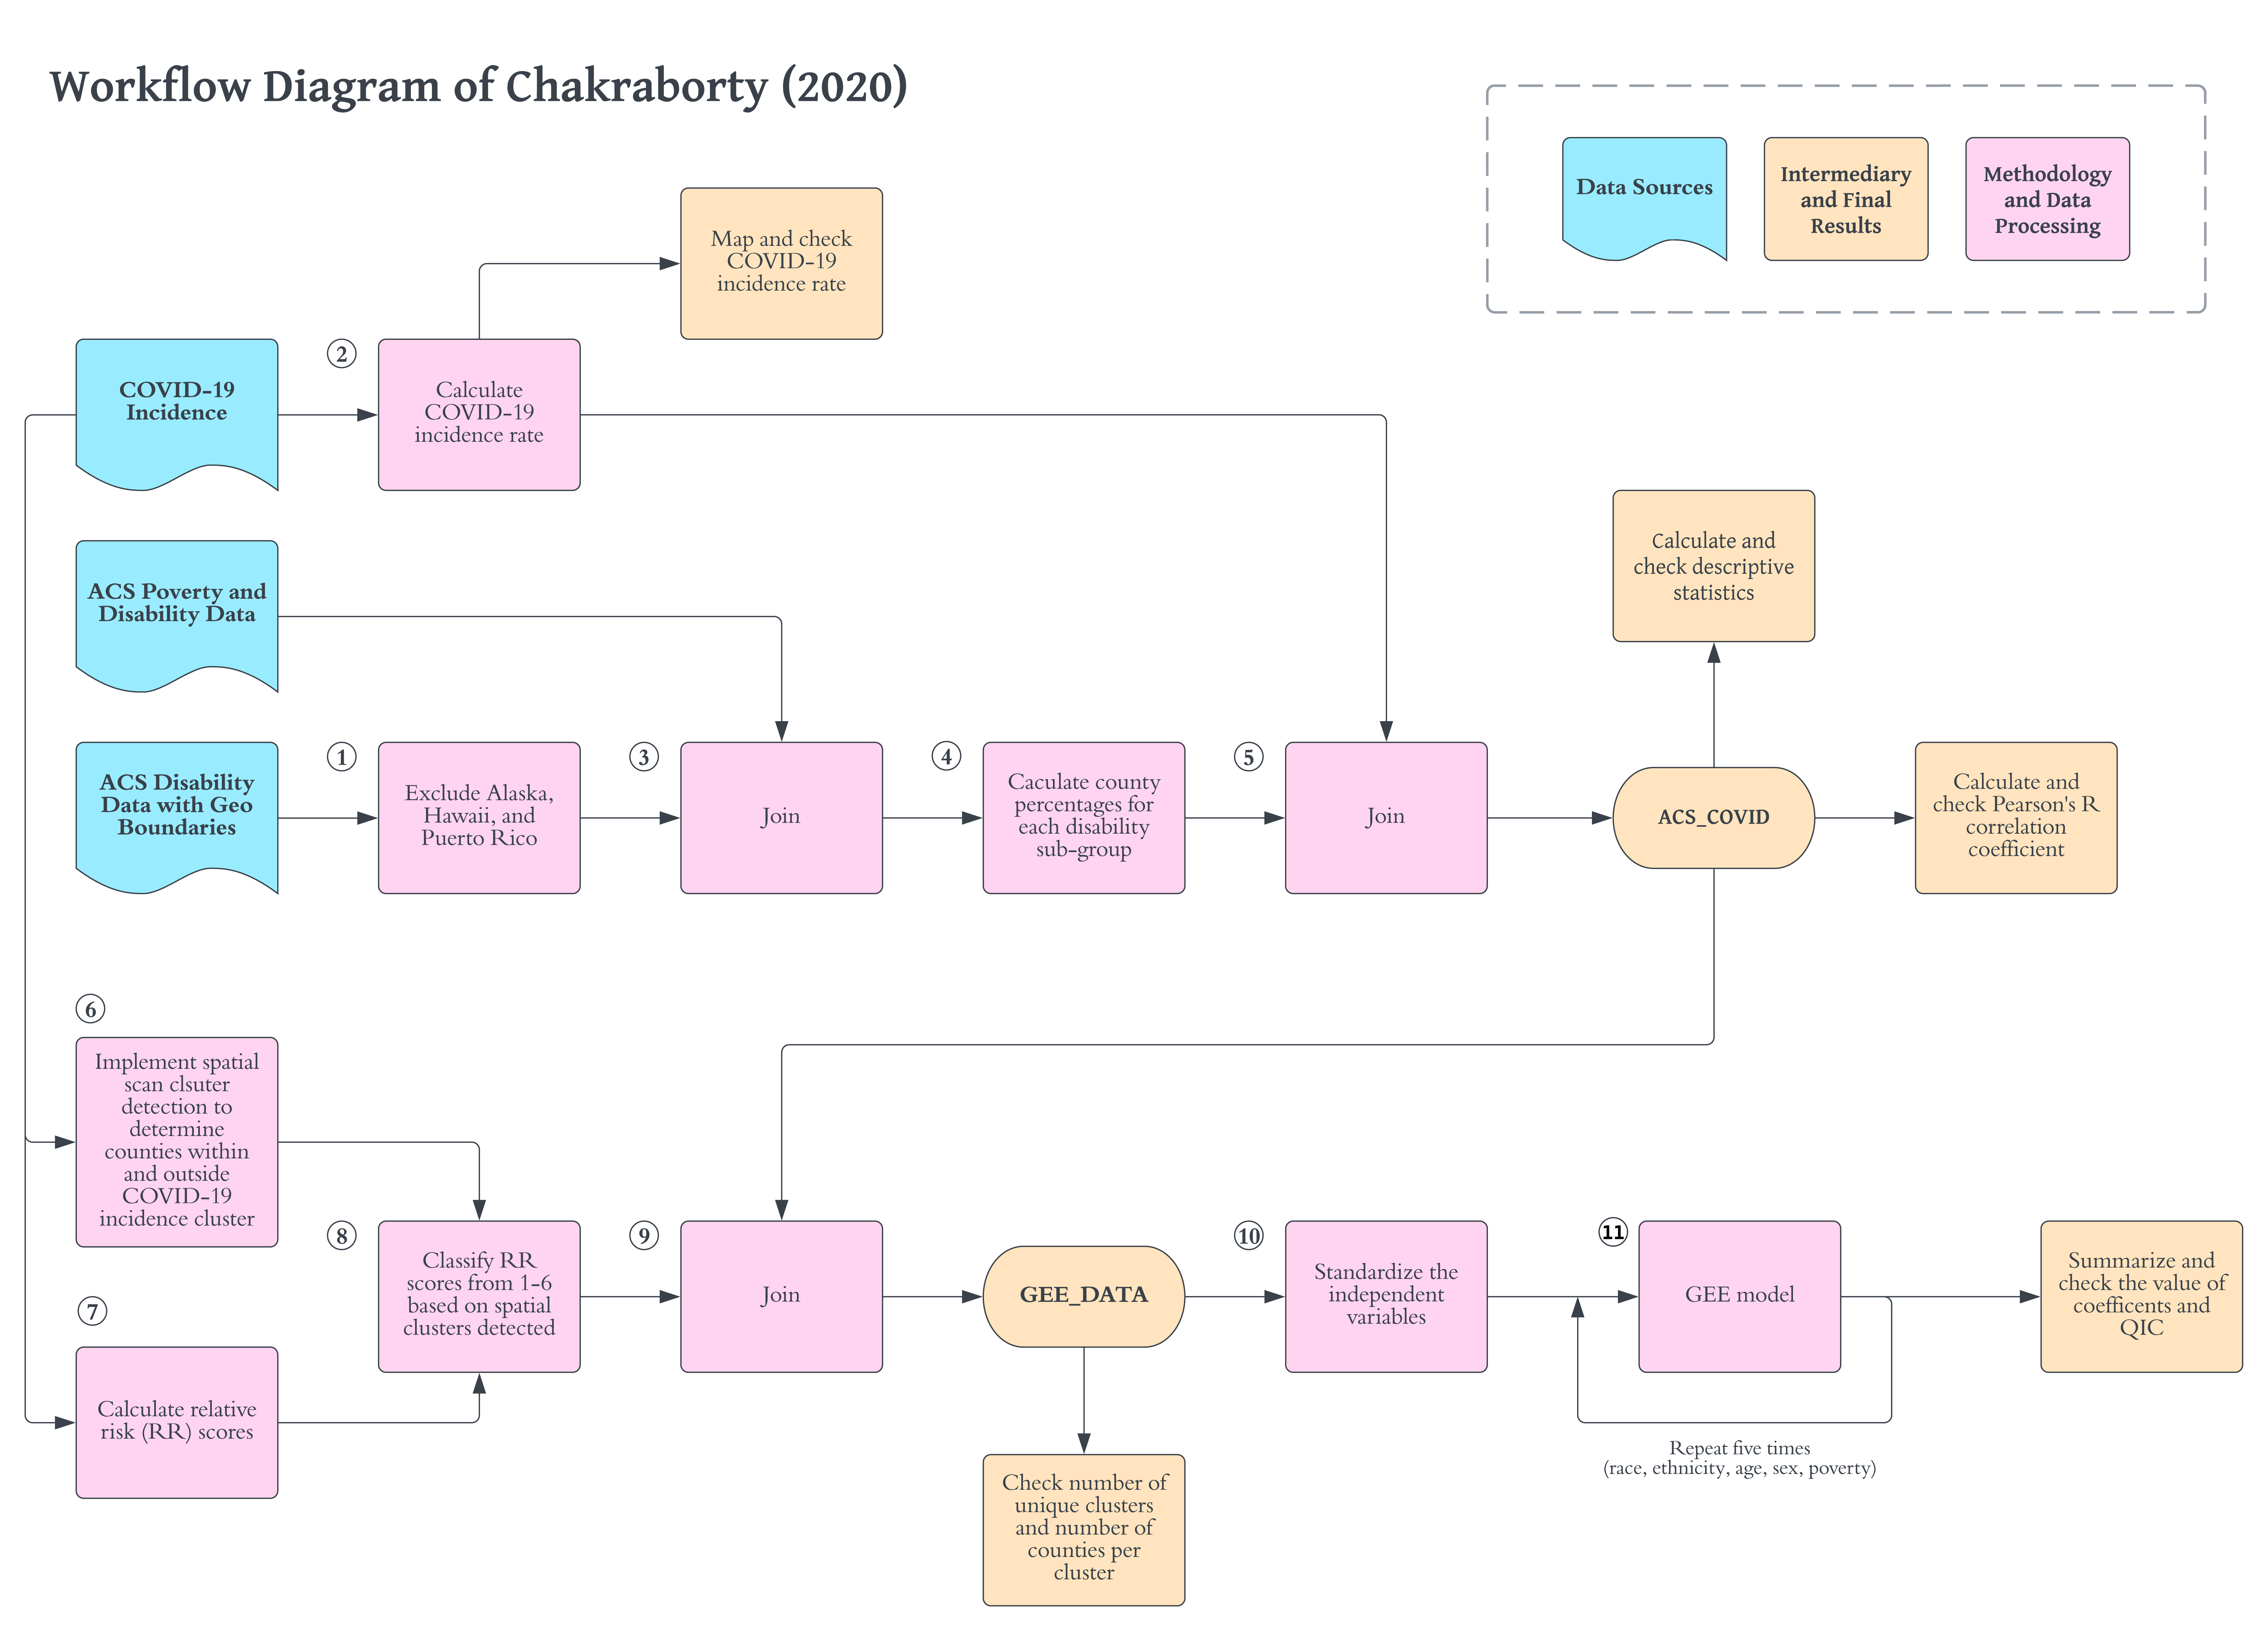
\includegraphics{../../docs/report/workflow.jpg}

\hypertarget{computational-environment}{%
\section{Computational environment}\label{computational-environment}}

The study was originally conducted using SaTScan software to implement
the Kulldorff spatial scan statistic. Other software are not specified
in the publication; however data files suggest and communication with
the author verifies that spatial analysis and mapping was conducted in
ArcGIS, generalized estimating equation (GEE) models were calculated in
SPSS, and the SaTScan software version was \texttt{9.6}.

This reproduction study uses R, including the SpatialEpi package for the
Kulldorff spatial scan statistics and the geepack package for GEE
models.

\hypertarget{data}{%
\section{Data}\label{data}}

\hypertarget{acs-socio-demographic-data}{%
\subsection{ACS Socio-demographic
data}\label{acs-socio-demographic-data}}

The American Community Survey (ACS) five-year estimate (2014-2018)
variables used in the study are outlined in the table below. Details on
ACS data collection can be found at
\url{https://www.census.gov/topics/health/disability/guidance/data-collection-acs.html}
and details on sampling methods and accuracy can be found at
\url{https://www.census.gov/programs-surveys/acs/technical-documentation/code-lists.html}.

\begin{longtable}[]{@{}
  >{\centering\arraybackslash}p{(\columnwidth - 2\tabcolsep) * \real{0.5000}}
  >{\centering\arraybackslash}p{(\columnwidth - 2\tabcolsep) * \real{0.5000}}@{}}
\caption{Disability Subgroup Variables}\tabularnewline
\toprule\noalign{}
\begin{minipage}[b]{\linewidth}\centering
Variable Name in Study
\end{minipage} & \begin{minipage}[b]{\linewidth}\centering
ACS Variable name
\end{minipage} \\
\midrule\noalign{}
\endfirsthead
\toprule\noalign{}
\begin{minipage}[b]{\linewidth}\centering
Variable Name in Study
\end{minipage} & \begin{minipage}[b]{\linewidth}\centering
ACS Variable name
\end{minipage} \\
\midrule\noalign{}
\endhead
\bottomrule\noalign{}
\endlastfoot
percent of total civilian non-institutionalized population with a
disability & S1810\_C03\_001E \\
\textbf{Race} & \\
percent w disability: White alone & S1810\_C03\_004E \\
percent w disability: Black alone & S1810\_C03\_005E \\
percent w disability: Native American & S1810\_C03\_006E \\
percent w disability: Asian alone & S1810\_C03\_007E \\
percent w disability: Other race & S1810\_C03\_009E \\
\textbf{Ethnicity} & \\
percent w disability: Non-Hispanic White & S1810\_C03\_0011E \\
percent w disability: Hispanic & S1810\_C03\_012E \\
percent w disability: Non-Hispanic non-White & (S1810\_C02\_001E -
S1810\_C02\_011E - S1810\_C02\_012E) / (S1810\_C01\_001E -
S1810\_C01\_011E - S1810\_C01\_012E) * 100 \\
percent w disability: Other race & S1810\_C03\_009E \\
\textbf{Poverty} & \\
percent w disability: Below poverty level & (C18130\_004E + C18130\_011E
+ C18130\_018E) / C18130\_001E * 100 \\
percent w disability: Above poverty level & (C18130\_005E + C18130\_012E
+ C18130\_019E) / C18130\_001E * 100 \\
\textbf{Age} & \\
percent w disability: 5-17 & S1810\_C03\_014E \\
percent w disability: 18-34 & S1810\_C03\_015E \\
percent w disability: 35-64 & S1810\_C03\_016E \\
percent w disability: 65-74 & S1810\_C03\_017E \\
percent w disability: 75+ & S1810\_C03\_018E \\
\textbf{Biological sex} & \\
percent w disability: male & S1810\_C03\_001E \\
percent w disability: female & S1810\_C03\_003E \\
\end{longtable}

American Community Survey (ACS) data for sociodemographic subcategories
of people with disabilities can be accessed by using the
\texttt{tidycensus} package to query the Census API. This requires an
API key which can be acquired at
\href{https://api.census.gov/data/key_signup.html}{api.census.gov/data/key\_signup.html}.

\hypertarget{acs-data-transformations}{%
\subsubsection{ACS data
transformations}\label{acs-data-transformations}}

The original study extent is the lower 48 states and Washington D.C.
Therefore, Alaska, Hawai'i and Puerto Rico are removed from the data
(workflow step 1). Data on people with disabilities in poverty is
derived from a different census table (C18130) than data on people with
disabilities and age, race, ethnicity, age, and biological sex (S1810).
Therefore, join the poverty data to the other data using the GEOID
(workflow step 3). Also transform the ACS geographic data into
Contiguous USA Albers Equal Area projection and fix geometry errors.

Optionally, save the raw ACS data to \texttt{data/raw/public/acs.gpkg}
for use in GIS software.

Calculate independent socio-demographic variables of people with
disabilities as percentages for each sub-category of disability (race,
ethnicity, poverty, age, and biological sex) and remove raw census data
from the data frame (workflow step 4). Reproject the data into an Albers
equal area conic projection.

\hypertarget{covid-19-data}{%
\subsection{COVID-19 data}\label{covid-19-data}}

Data on COVID-19 cases from the Johns Hopkins University dashboard have
been provided directly with the research compendium because the data is
no longer available online in the state in which it was downloaded on
August 1, 2020. The dashboard and cumulative counts of COVID-19 cases
and deaths were continually updated, so an exact reproduction required
communication with the original author, Jayajit Chakraborty, for
assistance with provision of data from August 1, 2020. The data includes
an estimate of the total population (\texttt{POP\_ESTIMA}) and confirmed
COVID-19 cases (\texttt{Confirmed}). The COVID-19 case data expresses
cumulative count of reported COVID-19 from 1/22/2020 to 8/1/2020.
Although metadata for this particular resource is no longer available
from the original source, one can reasonably assume that the total
population estimate was based on the 2014-2018 5-year ACS estimate, as
the 2019 estimates data had not been released yet.

Versions of the data can be found at the John Hopkins CCSE COVID-19 Data
Repository (\url{https://github.com/CSSEGISandData/COVID-19}). However,
archived data only provides summaries at the national scale. We received
the COVID-19 case data through 8/1/2020 at the county level from the
author, as there is no readily apparent way to access archived data from
the Johns Hopkins University Center for Systems Science Engineering
database.

\hypertarget{covid-19-data-transformations}{%
\subsubsection{COVID-19 data
transformations}\label{covid-19-data-transformations}}

Calculate the COVID incidence rate as the cases per 100,000 people
(workflow step 2). Convert the COVID data to a non-geographic data
frame.

Join dependent COVID data to independent ACS demographic data.

\hypertarget{missing-data}{%
\subsection{Missing data}\label{missing-data}}

\textbf{Unplanned deviation for reproduction}: There is one county with
missing disability and poverty data. This was not mentioned in the
original study or in our pre-analyis plan. However, we replace the
missing data with zeros, producing results identical to Chakraborty's.

\begin{tabular}{l|l|l|l|r|r|r|r|r|r|r|r|r|r|r|r|r|r|r|r|r|r|r|r|r|r|r}
\hline
fips & statefp & county & county\_st & covid\_rate & dis\_pct & white\_pct & black\_pct & native\_pct & asian\_pct & other\_pct & non\_hisp\_white\_pct & hisp\_pct & non\_hisp\_non\_white\_pct & bpov\_pct & apov\_pct & pct\_5\_17 & pct\_18\_34 & pct\_35\_64 & pct\_65\_74 & pct\_75 & male\_pct & female\_pct & pop & cases & x & y\\
\hline
35039 & 35 & Rio Arriba & Rio Arriba County, New Mexico & 751.17 & 16.06467 & 10.77458 & 0.038371 & 2.744807 & 0.038371 & 2.468536 & 2.355981 & 11.39619 & 2.312494 & NA & NA & 0.3069682 & 1.258569 & 6.781439 & 3.391998 & 4.279648 & 8.556738 & 7.50793 & 39006 & 293 & -106.6932 & 36.50962\\
\hline
\end{tabular}

\hypertarget{map-covid-19-incidence}{%
\subsection{Map COVID-19 incidence}\label{map-covid-19-incidence}}

Map the county level distribution of COVID-19 incidence rates, comparing
to Figure 1 of the original study.

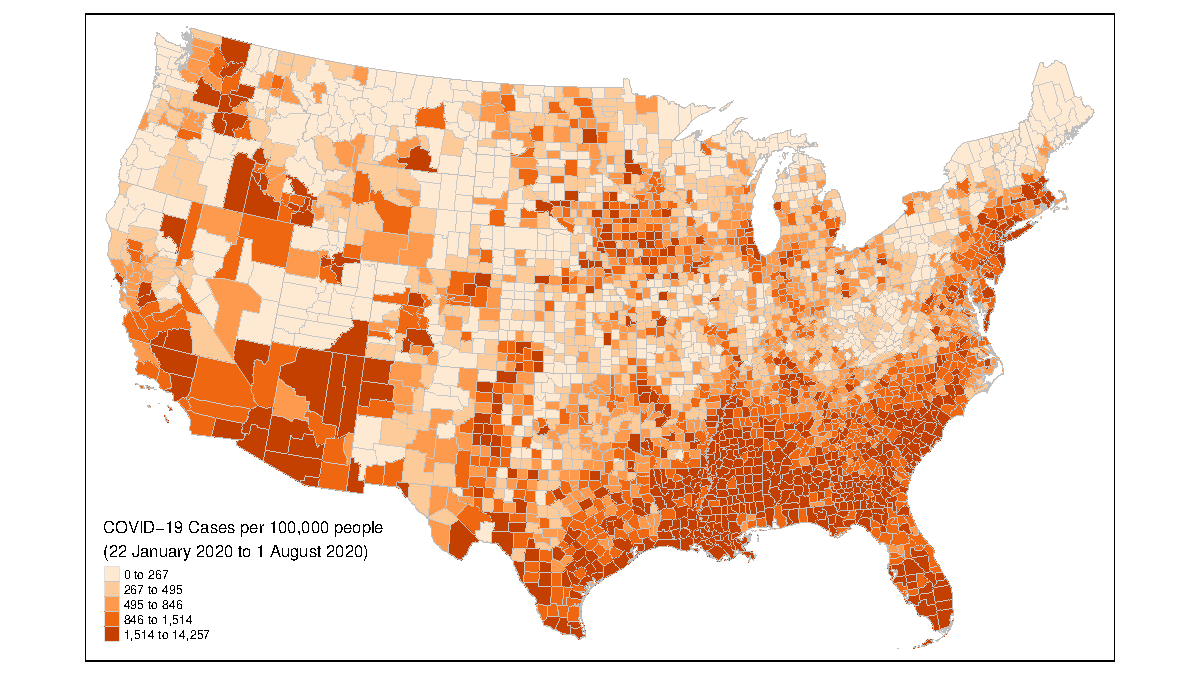
\includegraphics{C:/Users/gshanleybarr/Desktop/RPr-Chakraborty-2021/results/figures/map-covid-rates-1.pdf}

\hypertarget{map-disability-rates}{%
\subsection{Map disability rates}\label{map-disability-rates}}

\textbf{Unplanned deviation for reproduction}: We also map the spatial
distribution of the percent of people with any disability to improve our
understanding of the geographic patterns and relationships of between
the overarching independent variable (percentage of people with
disability) and the dependent variable (COVID-19 incidence rate).

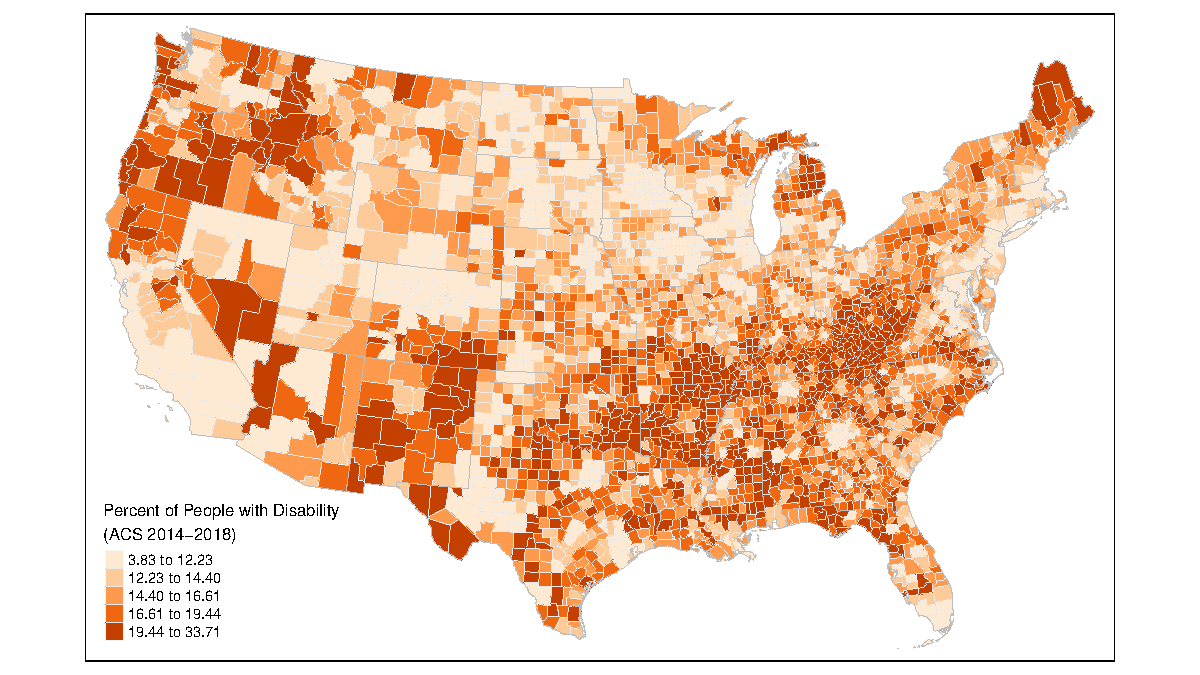
\includegraphics{C:/Users/gshanleybarr/Desktop/RPr-Chakraborty-2021/results/figures/map-disability-rates-1.pdf}

\hypertarget{descriptive-statistics}{%
\subsection{Descriptive statistics}\label{descriptive-statistics}}

Calculate descriptive statistics for dependent COVID-19 rate and
independent socio-demographic characteristics, reproducing the min, max,
mean, and SD columns of original study table 1.

\textbf{Planned deviation for reanalysis}: We also calculate the Shapiro
Wilk test for normality.

\begin{table}

\caption{\label{tab:descriptive-statistics}Reproduced Descriptive Statistics}
\centering
\begin{tabular}[t]{l|>{}c|>{}c|>{}c|>{}c|>{}c|>{}c}
\hline
  & min & max & mean & SD & ShapiroWilk & p\\
\hline
covid\_rate & 0.00 & 14257.17 & 966.90 & 1003.96 & 0.74 & 0\\
\hline
dis\_pct & 3.83 & 33.71 & 15.95 & 4.40 & 0.98 & 0\\
\hline
white\_pct & 0.85 & 33.26 & 13.55 & 4.63 & 0.98 & 0\\
\hline
black\_pct & 0.00 & 20.70 & 1.48 & 2.66 & 0.61 & 0\\
\hline
native\_pct & 0.00 & 13.74 & 0.28 & 0.94 & 0.28 & 0\\
\hline
asian\_pct & 0.00 & 3.45 & 0.09 & 0.18 & 0.51 & 0\\
\hline
other\_pct & 0.00 & 15.24 & 0.55 & 0.65 & 0.57 & 0\\
\hline
non\_hisp\_white\_pct & 0.10 & 33.16 & 12.84 & 4.81 & 0.99 & 0\\
\hline
hisp\_pct & 0.00 & 25.26 & 0.99 & 2.15 & 0.42 & 0\\
\hline
non\_hisp\_non\_white\_pct & 0.00 & 20.93 & 2.13 & 2.75 & 0.70 & 0\\
\hline
bpov\_pct & 0.00 & 14.97 & 3.57 & 1.85 & 0.93 & 0\\
\hline
apov\_pct & 0.00 & 27.30 & 12.48 & 3.06 & 0.99 & 0\\
\hline
pct\_5\_17 & 0.00 & 5.08 & 1.03 & 0.48 & 0.95 & 0\\
\hline
pct\_18\_34 & 0.00 & 5.59 & 1.56 & 0.67 & 0.96 & 0\\
\hline
pct\_35\_64 & 1.01 & 18.36 & 6.35 & 2.30 & 0.96 & 0\\
\hline
pct\_65\_74 & 0.00 & 12.73 & 3.09 & 1.16 & 0.95 & 0\\
\hline
pct\_75 & 0.00 & 11.13 & 3.87 & 1.19 & 0.97 & 0\\
\hline
male\_pct & 1.30 & 18.19 & 8.06 & 2.37 & 0.98 & 0\\
\hline
female\_pct & 1.91 & 19.94 & 7.90 & 2.26 & 0.98 & 0\\
\hline
\end{tabular}
\end{table}

Compare reproduced descriptive statistics to original descriptive
statistics. Difference is calculated as `reproduction study - original
study'. Identical results will result in zero.

\begin{table}

\caption{\label{tab:compare-descriptive-stats}Descriptive Statistics Comparison}
\centering
\begin{tabular}[t]{l|>{\centering\arraybackslash}p{4em}|>{\centering\arraybackslash}p{4em}|>{\centering\arraybackslash}p{4em}|>{\centering\arraybackslash}p{4em}}
\hline
  & min & max & mean & SD\\
\hline
covid\_rate & 0 & 0.17 & -0.1 & -0.04\\
\hline
dis\_pct & 0 & 0.00 & 0.0 & 0.00\\
\hline
white\_pct & 0 & 0.00 & 0.0 & 0.00\\
\hline
black\_pct & 0 & 0.00 & 0.0 & 0.00\\
\hline
native\_pct & 0 & 0.00 & 0.0 & 0.00\\
\hline
asian\_pct & 0 & 0.00 & 0.0 & 0.00\\
\hline
other\_pct & 0 & 0.00 & 0.0 & 0.00\\
\hline
non\_hisp\_white\_pct & 0 & 0.00 & 0.0 & 0.00\\
\hline
hisp\_pct & 0 & 0.00 & 0.0 & 0.00\\
\hline
non\_hisp\_non\_white\_pct & 0 & 0.00 & 0.0 & 0.00\\
\hline
bpov\_pct & 0 & 0.00 & 0.0 & 0.00\\
\hline
apov\_pct & 0 & 0.00 & 0.0 & 0.00\\
\hline
pct\_5\_17 & 0 & 0.00 & 0.0 & 0.00\\
\hline
pct\_18\_34 & 0 & 0.00 & 0.0 & 0.00\\
\hline
pct\_35\_64 & 0 & 0.00 & 0.0 & 0.00\\
\hline
pct\_65\_74 & 0 & 0.00 & 0.0 & 0.00\\
\hline
pct\_75 & 0 & 0.00 & 0.0 & 0.00\\
\hline
male\_pct & 0 & 0.00 & 0.0 & 0.00\\
\hline
female\_pct & 0 & 0.00 & 0.0 & 0.00\\
\hline
\end{tabular}
\end{table}

The descriptive statistics are identical, except that the original study
seems to have rounded the COVID-19 statistics to zero decimal places.

\hypertarget{analytical-methods}{%
\section{Analytical methods}\label{analytical-methods}}

\hypertarget{bivariate-parametric-correlation-analysis}{%
\subsection{Bivariate parametric correlation
analysis}\label{bivariate-parametric-correlation-analysis}}

The county-level Pearson's rho correlation coefficient was used to test
association between intra-categorical rates of disability and COVID-19
incidence rates. As this was a parametric test, normality should be
tested. A separate hypothesis was formulated for disability in aggregate
and for each sociodemographic disability characteristic.

Calculate Pearson's R Correlation Coefficient of each independent
variable and the COVID-19 incidence rate, reproducing the Pearson's R
column of original study Table 1.

\begin{table}

\caption{\label{tab:pearsons-correlation}Reproduced Pearson's R}
\centering
\begin{tabular}[t]{c|>{\centering\arraybackslash}p{4em}|>{\centering\arraybackslash}p{4em}|>{\centering\arraybackslash}p{4em}}
\hline
variable & r & t & p\\
\hline
dis\_pct & -0.060 & 3.350 & 0.000\\
\hline
white\_pct & -0.332 & 19.612 & 0.000\\
\hline
black\_pct & 0.460 & 28.847 & 0.000\\
\hline
native\_pct & 0.019 & 1.072 & 0.142\\
\hline
asian\_pct & 0.094 & 5.272 & 0.000\\
\hline
other\_pct & 0.026 & 1.460 & 0.072\\
\hline
non\_hisp\_white\_pct & -0.361 & 21.545 & 0.000\\
\hline
hisp\_pct & 0.119 & 6.686 & 0.000\\
\hline
non\_hisp\_non\_white\_pct & 0.442 & 27.429 & 0.000\\
\hline
bpov\_pct & 0.106 & 5.914 & 0.000\\
\hline
apov\_pct & -0.151 & 8.513 & 0.000\\
\hline
pct\_5\_17 & 0.084 & 4.688 & 0.000\\
\hline
pct\_18\_34 & 0.063 & 3.493 & 0.000\\
\hline
pct\_35\_64 & -0.008 & 0.460 & 0.323\\
\hline
pct\_65\_74 & -0.091 & 5.113 & 0.000\\
\hline
pct\_75 & -0.186 & 10.541 & 0.000\\
\hline
male\_pct & -0.134 & 7.519 & 0.000\\
\hline
female\_pct & 0.023 & 1.305 & 0.096\\
\hline
pop & 0.128 & 7.215 & 0.000\\
\hline
cases & 0.209 & 11.891 & 0.000\\
\hline
x & 0.099 & 5.540 & 0.000\\
\hline
y & -0.412 & 25.195 & 0.000\\
\hline
\end{tabular}
\end{table}

Compare the reproduced Pearson's \emph{r} correlation coefficients to
the original study's Pearson's \emph{r} correlation coefficients. Stars
indicates the significance level with two stars for
\texttt{p\ \textless{}\ 0.01} and one star for
\texttt{p\ \textless{}\ 0.05}. Correlation difference
\texttt{rp\_r\_diff} is calculated between the reproduction study
\texttt{rp\_r} and original study \texttt{or\_r} as
\texttt{rp\_r\_diff\ =\ rp\_r\ -\ or\_r} Direction difference
\texttt{rp\_dir\_diff} is calculated as
\texttt{(rp\_r\ \textgreater{}\ 0)\ -\ (or\_r\ \textgreater{}\ 0)},
giving \texttt{0} if both coefficients have the same direction,
\texttt{1} if the reproduction is positive and the original is negative,
and \texttt{-1} if the reproduction is negative but the original is
positive.

\begin{table}

\caption{\label{tab:compare-pearsons-correlation}Compare reproduced and original Pearson's R}
\centering
\begin{tabular}[t]{c|c|c|c|c|c|c|c}
\hline
\multicolumn{1}{c|}{ } & \multicolumn{2}{c|}{Original} & \multicolumn{2}{c|}{Reproduced} & \multicolumn{3}{c}{Difference} \\
\cline{2-3} \cline{4-5} \cline{6-8}
Variable & R & Sig. Level & R & Sig. Level & R & Sig. Level & Direction\\
\hline
dis\_pct & -0.056 & 2 & -0.060 & 2 & -0.004 & 0 & 0\\
\hline
white\_pct & -0.326 & 2 & -0.332 & 2 & -0.006 & 0 & 0\\
\hline
black\_pct & 0.456 & 2 & 0.460 & 2 & 0.004 & 0 & 0\\
\hline
native\_pct & 0.020 & 0 & 0.019 & 0 & -0.001 & 0 & 0\\
\hline
asian\_pct & 0.097 & 2 & 0.094 & 2 & -0.003 & 0 & 0\\
\hline
other\_pct & 0.028 & 0 & 0.026 & 0 & -0.002 & 0 & 0\\
\hline
non\_hisp\_white\_pct & -0.355 & 2 & -0.361 & 2 & -0.006 & 0 & 0\\
\hline
hisp\_pct & 0.119 & 2 & 0.119 & 2 & 0.000 & 0 & 0\\
\hline
non\_hisp\_non\_white\_pct & 0.439 & 2 & 0.442 & 2 & 0.003 & 0 & 0\\
\hline
bpov\_pct & 0.108 & 2 & 0.106 & 2 & -0.002 & 0 & 0\\
\hline
apov\_pct & -0.146 & 2 & -0.151 & 2 & -0.005 & 0 & 0\\
\hline
pct\_5\_17 & 0.083 & 2 & 0.084 & 2 & 0.001 & 0 & 0\\
\hline
pct\_18\_34 & 0.066 & 1 & 0.063 & 2 & -0.003 & 1 & 0\\
\hline
pct\_35\_64 & -0.005 & 0 & -0.008 & 0 & -0.003 & 0 & 0\\
\hline
pct\_65\_74 & -0.089 & 2 & -0.091 & 2 & -0.002 & 0 & 0\\
\hline
pct\_75 & -0.181 & 2 & -0.186 & 2 & -0.005 & 0 & 0\\
\hline
male\_pct & -0.131 & 2 & -0.134 & 2 & -0.003 & 0 & 0\\
\hline
female\_pct & 0.028 & 0 & 0.023 & 0 & -0.005 & 0 & 0\\
\hline
\end{tabular}
\end{table}

Reproduction correlation coefficients varied slightly from the original
study coefficients by +/- 0.006. All but one Pearson's correlation
coefficient was significant to the same level, and the exception was age
18 to 34. Counter-intuitively, the correlation coefficient was slightly
closer to 0 but the \emph{p} value was also found to be more
significant, suggesting a difference in the estimation of \emph{t}
and/or \emph{p}, or a typographical error. All of the coefficients had
the same direction.

\textbf{Unplanned Deviation for Reproduction}: We should expect
identical results for this correlation test, so we loaded the original
author's data from \texttt{Aug1GEEdata.csv} to re-test the statistic,
calculated as \texttt{unplanned\_r} below.

\begin{table}

\caption{\label{tab:original-data-pearson-correlation}Recalculation of Pearson's R with original data}
\centering
\begin{tabular}[t]{c|c|c|c}
\hline
variable & unplanned\_r & or\_r & diff\\
\hline
dis\_pct & -0.056 & -0.056 & 0\\
\hline
white\_pct & -0.326 & -0.326 & 0\\
\hline
black\_pct & 0.456 & 0.456 & 0\\
\hline
native\_pct & 0.020 & 0.020 & 0\\
\hline
asian\_pct & 0.097 & 0.097 & 0\\
\hline
other\_pct & 0.028 & 0.028 & 0\\
\hline
non\_hisp\_white\_pct & -0.355 & -0.355 & 0\\
\hline
hisp\_pct & 0.119 & 0.119 & 0\\
\hline
non\_hisp\_non\_white\_pct & 0.439 & 0.439 & 0\\
\hline
bpov\_pct & 0.108 & 0.108 & 0\\
\hline
apov\_pct & -0.146 & -0.146 & 0\\
\hline
pct\_5\_17 & 0.083 & 0.083 & 0\\
\hline
pct\_18\_34 & 0.066 & 0.066 & 0\\
\hline
pct\_35\_64 & -0.005 & -0.005 & 0\\
\hline
pct\_65\_74 & -0.089 & -0.089 & 0\\
\hline
pct\_75 & -0.181 & -0.181 & 0\\
\hline
male\_pct & -0.131 & -0.131 & 0\\
\hline
female\_pct & 0.028 & 0.028 & 0\\
\hline
\end{tabular}
\end{table}

The author's original data produced coefficients identical to the
original publication! Is it possible that the data values are correct
but have been reassigned / transposed to different counties?

\emph{Unplanned Deviation for Reproduction}: Considering the precise
bitwise reproduction of descriptive statistics and of correlation
statistics from author-provided data, we decided to recalculate the
COVID-19 incidence rate with author-provided case and population data
for comparison to the author-provided incidence rate.

\begin{table}

\caption{\label{tab:compare-incidence-rate}Counties with inconsistent COVID-19 incidence rate}
\centering
\resizebox{\linewidth}{!}{
\begin{tabular}[t]{r|l|l|r|r|r|r|r}
\hline
FIPS & State & County & Population & Cases & OR\_Incidence & RPr\_Incidence & Difference\\
\hline
1115 & Alabama & St. Clair & 88690 & 1151 & 1349.52 & 1297.78 & -51.74\\
\hline
1117 & Alabama & Shelby & 215707 & 2911 & 1297.78 & 1349.52 & 51.74\\
\hline
5123 & Arkansas & St. Francis & 25439 & 1112 & 704.16 & 4371.24 & 3667.08\\
\hline
5125 & Arkansas & Saline & 121421 & 855 & 397.33 & 704.16 & 306.83\\
\hline
5127 & Arkansas & Scott & 10319 & 41 & 314.15 & 397.33 & 83.18\\
\hline
5129 & Arkansas & Searcy & 7958 & 25 & 1322.08 & 314.15 & -1007.93\\
\hline
5131 & Arkansas & Sebastian & 127753 & 1689 & 5420.39 & 1322.08 & -4098.31\\
\hline
5133 & Arkansas & Sevier & 17139 & 929 & 570.08 & 5420.39 & 4850.31\\
\hline
5135 & Arkansas & Sharp & 17366 & 99 & 4371.24 & 570.08 & -3801.16\\
\hline
8039 & Colorado & Elbert & 26282 & 85 & 626.60 & 323.42 & -303.18\\
\hline
8041 & Colorado & El Paso & 713856 & 4473 & 323.42 & 626.60 & 303.18\\
\hline
8065 & Colorado & Lake & 7824 & 70 & 349.85 & 894.68 & 544.83\\
\hline
8067 & Colorado & La Plata & 56310 & 197 & 894.68 & 349.85 & -544.83\\
\hline
\end{tabular}}
\end{table}

We found that 13 counties had incorrect COVID-19 incidence scores, and
the scores seem to be transposed from other counties, such that the
overall descriptive statistics were accurate but the correlation
coefficients were inaccurate. This finding implies that subsequent
analyses using the COVID-19 Incidence rate will be slightly different
and more accurate in this reproduction study than in the original study.

\textbf{Unplanned deviation for reproduction:} Join the original
author's Incidence data into our reproduction data frame so that we can
later test for sensitivity to this error. Then report any counties for
which the reproduced COVID incidence rate differs from the original
author's COVID incidence rate.

\begin{table}

\caption{\label{tab:join-incidence-rate}Original incidence rate joined to reproduction data}
\centering
\begin{tabular}[t]{l|r|r}
\hline
county\_st & covid\_rate & or\_incidence\\
\hline
St. Clair County, Alabama & 1297.78 & 1349.52\\
\hline
Shelby County, Alabama & 1349.52 & 1297.78\\
\hline
St. Francis County, Arkansas & 4371.24 & 704.16\\
\hline
Saline County, Arkansas & 704.16 & 397.33\\
\hline
Scott County, Arkansas & 397.33 & 314.15\\
\hline
Searcy County, Arkansas & 314.15 & 1322.08\\
\hline
Sebastian County, Arkansas & 1322.08 & 5420.39\\
\hline
Sevier County, Arkansas & 5420.39 & 570.08\\
\hline
Sharp County, Arkansas & 570.08 & 4371.24\\
\hline
Elbert County, Colorado & 323.42 & 626.60\\
\hline
El Paso County, Colorado & 626.60 & 323.42\\
\hline
Lake County, Colorado & 894.68 & 349.85\\
\hline
La Plata County, Colorado & 349.85 & 894.68\\
\hline
\end{tabular}
\end{table}

The join worked, highlighting the same 13 counties with inconsistent
incidence rates. This also confirms that our reproduced dependent
variable is identical to the original dependent variable with the
exception of these three counties.

\hypertarget{bivariate-nonparametric-correlation-analysis}{%
\subsection{Bivariate nonparametric correlation
analysis}\label{bivariate-nonparametric-correlation-analysis}}

\textbf{Unplanned Deviation for Reproduction}: The dependent and
independent variables in this study do not have normal distributions, as
shown in the Shapiro-Wilk test results above. Therefore, we deviate from
the original study to use the Spearman's Rho non-parametric correlation
test.

Compare the Spearman's \emph{rho} correlation coefficients to the
reproduced Pearson's \emph{r} correlation coefficients. Differences are
calculated as \emph{Spearman's Rho} - \emph{Pearson's R}.

\begin{table}
\centering
\begin{tabular}{c|c|c|c|c|c|c|c}
\hline
\multicolumn{1}{c|}{ } & \multicolumn{2}{c|}{Pearson's} & \multicolumn{2}{c|}{Spearman's} & \multicolumn{3}{c}{Difference} \\
\cline{2-3} \cline{4-5} \cline{6-8}
Variable & R & Stars & Rho & Stars & Rho - R & Stars & Direction\\
\hline
dis\_pct & -0.060 & 2 & -0.113 & 2 & -0.053 & 0 & 0\\
\hline
white\_pct & -0.332 & 2 & -0.421 & 2 & -0.089 & 0 & 0\\
\hline
black\_pct & 0.460 & 2 & 0.575 & 2 & 0.115 & 0 & 0\\
\hline
native\_pct & 0.019 & 0 & -0.084 & 2 & -0.103 & 2 & -1\\
\hline
asian\_pct & 0.094 & 2 & 0.194 & 2 & 0.100 & 0 & 0\\
\hline
other\_pct & 0.026 & 0 & 0.104 & 2 & 0.078 & 2 & 0\\
\hline
non\_hisp\_white\_pct & -0.361 & 2 & -0.454 & 2 & -0.093 & 0 & 0\\
\hline
hisp\_pct & 0.119 & 2 & 0.231 & 2 & 0.112 & 0 & 0\\
\hline
non\_hisp\_non\_white\_pct & 0.442 & 2 & 0.481 & 2 & 0.039 & 0 & 0\\
\hline
bpov\_pct & 0.106 & 2 & 0.062 & 2 & -0.044 & 0 & 0\\
\hline
apov\_pct & -0.151 & 2 & -0.205 & 2 & -0.054 & 0 & 0\\
\hline
pct\_5\_17 & 0.084 & 2 & 0.079 & 2 & -0.005 & 0 & 0\\
\hline
pct\_18\_34 & 0.063 & 2 & 0.034 & 1 & -0.029 & -1 & 0\\
\hline
pct\_35\_64 & -0.008 & 0 & -0.020 & 0 & -0.012 & 0 & 0\\
\hline
pct\_65\_74 & -0.091 & 2 & -0.151 & 2 & -0.060 & 0 & 0\\
\hline
pct\_75 & -0.186 & 2 & -0.285 & 2 & -0.099 & 0 & 0\\
\hline
male\_pct & -0.134 & 2 & -0.201 & 2 & -0.067 & 0 & 0\\
\hline
female\_pct & 0.023 & 0 & -0.014 & 0 & -0.037 & 0 & -1\\
\hline
\end{tabular}
\end{table}

Three variables change significance levels, with \emph{Native American}
and \emph{Other} races gaining significance and \emph{age 18-34} losing
significance. Two correlations change direction, with both \emph{Native
American} race (illustrated in scatterplot below) and \emph{Female}
households switching from positive correlations to negative
correlations. Instabilities between the parametric and non-parametic
correlations arise from variables with very skewed distributions and/or
weak correlations at the county level. Some difference may also be
attributable to the 13 counties with data errors in the COVID-19
Incidence Rate. In such distributions, outlier observations have more
weight in the parametric Person's R test than in the non-parametric
Spearman's Rho test.

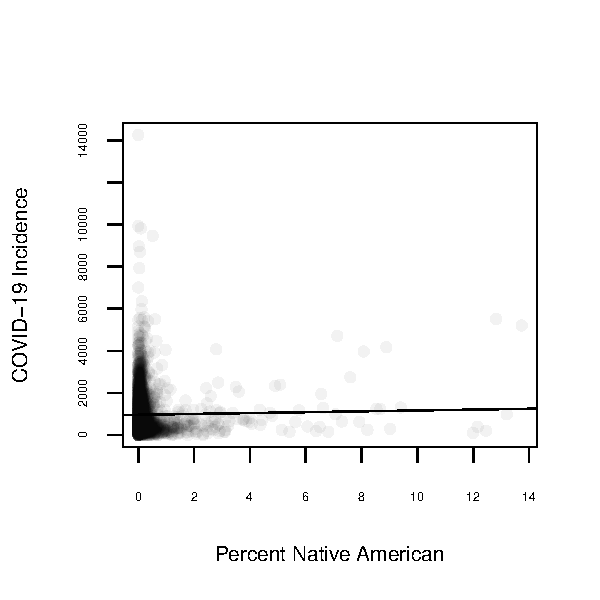
\includegraphics{C:/Users/gshanleybarr/Desktop/RPr-Chakraborty-2021/results/figures/plot-bivariate-1.pdf}

\hypertarget{kulldorff-spatial-scan-statistic}{%
\subsection{Kulldorff spatial scan
statistic}\label{kulldorff-spatial-scan-statistic}}

Although there were no major geographic \emph{transformations} in this
study, \emph{geographic grouping criteria} for the generalized
estimating equation (GEE) models are defined as a combination of states
and COVID-19 risk, which is based on the Kulldorff spatial scan
statistic for geographic clusters of high COVID-19 incidence. The scan
statistic in SaTScan used spherical great circle distance calculations
based upon the latitude and longitude coordinates of the centroid of
each county. For this purpose, we have used the \texttt{X} and
\texttt{Y} attributes provided as geographic variables with ACS data.

We use a Kulldorff spatial scan statistic to detect spatial clusters of
high COVID-19 incidence (workflow step 6). The statistic uses a Monte
Carlo simulation to calculate statistical significance, and therefore
may not produce identical results each time.

The original study uses SaTScan software to implement the Kulldorff
spatial scan statistic model. In SaTScan, models may be specified with
many parameters having significant implications for results. The
original manuscript only specifies that Poisson model should be used. We
can also intuit that the model is discrete (locations are stationary and
non-random), and spatial only (there is no temporal dimension). The
author-provided SaTScan results \texttt{SatScan\_results.txt} contains
additional parameters which appear to adhere closely to the software's
default settings. These include the maximum cluster size of ``50 percent
of population at risk'', and the ``GINI optimized cluster collection''
and ``no geographical overlap'' options for detecting secondary
clusters. The ``P-value Cutoff'' for significant clusters option did not
appear in the v9.6 output, suggesting that the software only allowed the
default ``no'' option for this at the time of the original study.

SaTScan software can also output two versions of geographic data:

\begin{itemize}
\tightlist
\item
  The \texttt{col} cluster polygon shapefile contains a circle for each
  cluster, where each polygon is a circle defined by the cluster center
  and radius. The attributes include a variable \texttt{REL\_RISK} for
  cluster relative risk
\item
  The \texttt{gis} location point shapefile contains one point for each
  county in a cluster. The attributes include variables \texttt{LOC\_RR}
  for local relative risk and \texttt{CLU\_RR} for cluster relative risk
\end{itemize}

The SaTScan software implementation of the Kulldorff spatial scan
statistic calculates two relative risk scores for locations:

\begin{itemize}
\tightlist
\item
  Cluster relative risk is the incidence rate of the population within
  the cluster divided by the incidence rate of the population outside of
  the cluster. This is calculated as \texttt{REL\_RISK} in the
  \texttt{col} cluster polygon shapefile and as \texttt{CLU\_RR} in the
  \texttt{gis} location point shapefile.
\item
  Local relative risk is the incidence rate of population within a
  location divided by the incidence rate of the population outside of
  the location. This is calculated as \texttt{LOC\_RR} in the
  \texttt{gis} location shapefile, and is not calculated in the
  \texttt{col} cluster polygon shapefile.
\end{itemize}

For the purposes of interpreting the spatial scan statistic, a
\emph{location} is a \emph{county centroid} while a \emph{cluster} is a
\emph{collection of counties} with high incidence rates, defined in the
shape of a circle with a \emph{center} location (a county centroid) and
a \emph{radius}.

The original study is not clear about using the cluster geographic data
\emph{vs} the location geographic data or the cluster relative risk
\emph{vs} local relative risk. However, The author-provided
\texttt{SatScan\_results.txt} results file indicates a geographic
cluster file but no location file, and the author-provided
\texttt{Aug1GEEdata.csv} data table contains a \texttt{REL\_RISK} field
but no \texttt{CLU\_RR} field or \texttt{LOC\_RR} field. This suggests
that in the original study, the \texttt{col} polygon cluster shapefile
and \emph{cluster} relative risk were used to represent COVID-19 risk
and define GEE clusters.

The spatial scan statistic is based on case counts and total population,
and is therefore unaffected by errors in the COVID Incidence rate.

\textbf{Planned deviation for reproduction}: We opted to use the
SpatialEpi package in R, selecting open source software with R
integration over SatSCan software, which is free but not open. The
Kulldorff spatial scan statistic model in SpatialEpi also supports a
discrete Poisson spatial model, and uses the GINI coefficient to select
secondary clusters with no geographical overlap that maximize the
difference between locations inside of clusters and locations outside of
clusters. We expected that this set of software options could reproduce
identical results compared to SaTScan.

First, calculate the Kulldorff spatial scan statistic using SpatialEpi.
Optionally, skip this code block due to long run times of more than 10
minutes.

Load pre-calculated Kulldorff spatial scan results. Alternatively, skip
or modify this code block to use your own version of the SpatialEpi
Kulldorff results.

Report Kulldorff spatial scan results.

\begin{verbatim}
## [1] Most likely cluster:
\end{verbatim}

\begin{verbatim}
## $location.IDs.included
##  [1] 1824 1835 1797 1818 1825 1749 1854 1742 1837 1747 1838  280 1760 1846 1756
## 
## $population
## [1] 16949211
## 
## $number.of.cases
## [1] 469091
## 
## $expected.cases
## [1] 233805.6
## 
## $SMR
## [1] 2.006329
## 
## $log.likelihood.ratio
## [1] 97983.07
## 
## $monte.carlo.rank
## [1] 1
## 
## $p.value
## [1] 0.001
\end{verbatim}

\begin{verbatim}
## [1] Number of Secondary clusters: 134
\end{verbatim}

The \texttt{SpatialEpi} implementation of Kulldorff spatial scan
statistics provides output in the form of hierarchical lists analogous
to the text output of SaTScan, but does not output a simple data frame
or tabular output analogous to the shapefiles from SaTScan. Therefore,
additional steps are required to append the Kulldorff scan results to
the \texttt{acs\_covid} simple features data frame. This can be done by
assigning unique cluster ID's to each county within a cluster. Clusters
include the county at the center of a cluster and all of the other
counties within the cluster radius. Therefore, we use the FIPS code of
the county at the center of each cluster as the unique cluster ID.

\hypertarget{map-kulldorff-clusters}{%
\subsubsection{Map Kulldorff clusters}\label{map-kulldorff-clusters}}

\textbf{Unplanned deviation for reproduction}: The original study does
not include visualizations of the spatial structure and distribution of
COVID-19 clusters.

First, we must join the Kulldorff spatial scan cluster IDs to the
acs\_covid simple features dataframe. Although this was planned in
workflow step 9, the order of operations between steps 9 and steps 7 and
8 is not important.

Next, calculate a new field \texttt{isCluster} to identify counties in
COVID-19 clusters. Additionally, distinguish between counties defining
the center of a cluster from counties constituting other parts of a
cluster by comparing the cluster ID (equivalent to the center county's
fips code) to the county fips code.

\textbf{Planned deviation for reproduction}: Map the \texttt{SpatialEpi}
cluster results.

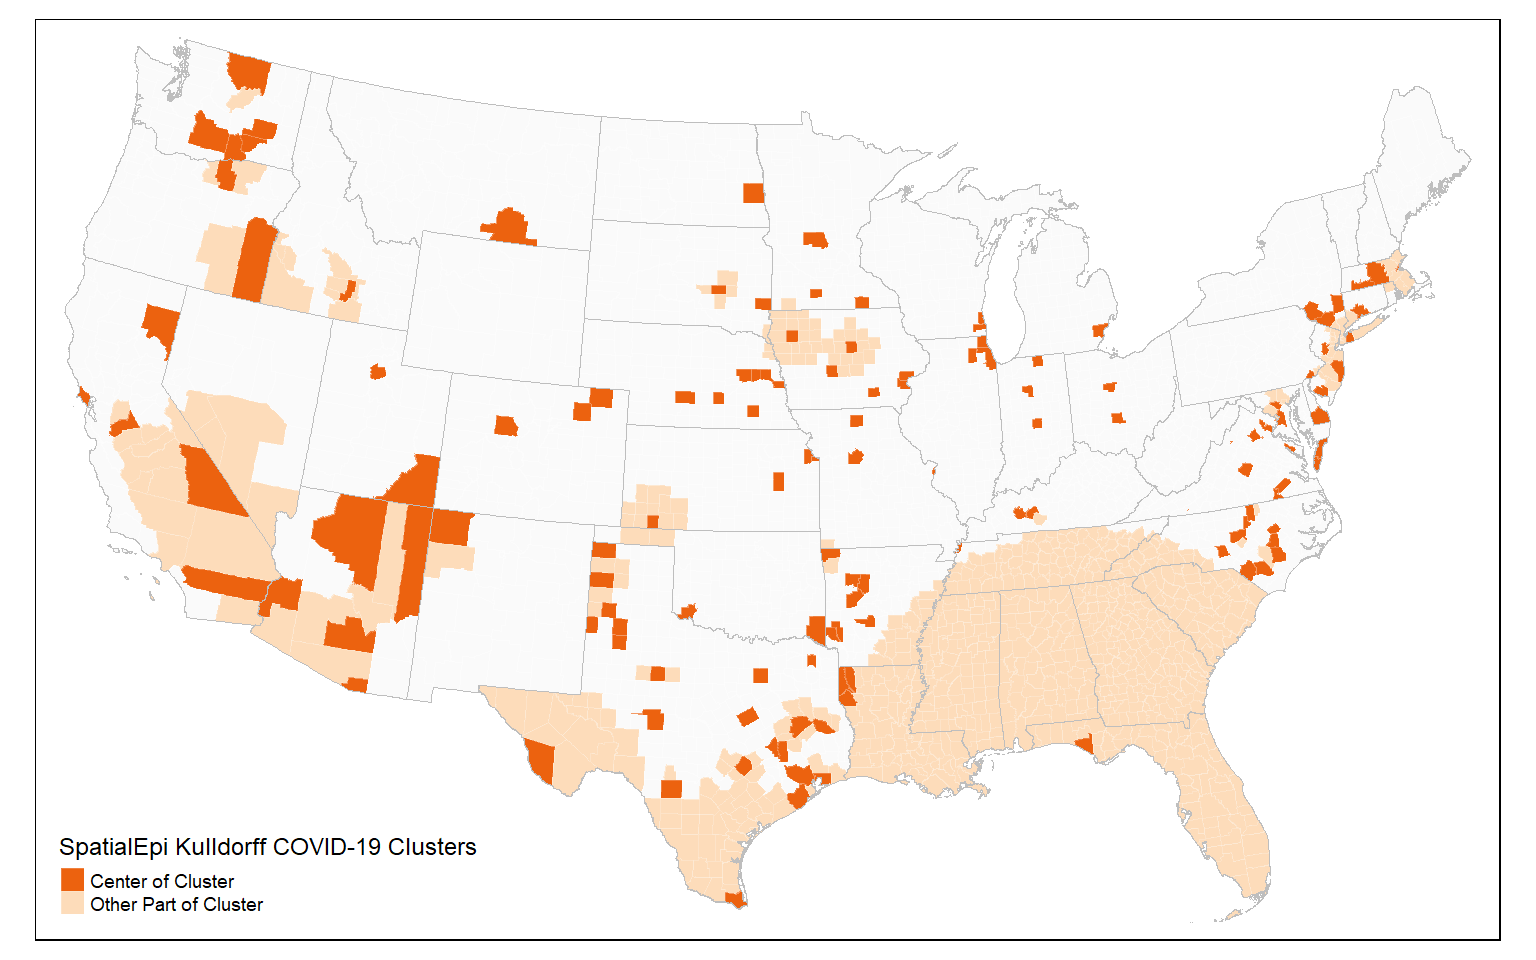
\includegraphics{C:/Users/gshanleybarr/Desktop/RPr-Chakraborty-2021/results/figures/map-clusters-1.pdf}

\textbf{Unplanned deviation for reproduction}: The \texttt{SpatialEpi}
implementation of Kulldorff spatial scan statistics does not calculate
local relative risk or cluster relative risk. Therefore, the next step
is to calculate local and cluster relative risk (workflow step 7).

Classify relative risk on a scale from 1 to 6 (workflow step 8). Risk is
classified according to this table:

\begin{longtable}[]{@{}cc@{}}
\toprule\noalign{}
Relative Risk Values & Relative Risk Class \\
\midrule\noalign{}
\endhead
\bottomrule\noalign{}
\endlastfoot
Outside of cluster & 1 \\
RR \textless{} 1 & 1 \\
1 \textless= RR \textless{} 2 & 2 \\
2 \textless= RR \textless{} 3 & 3 \\
3 \textless= RR \textless{} 4 & 4 \\
4 \textless= RR \textless{} 5 & 5 \\
5 \textless= RR \textless{} 6 & 6 \\
\end{longtable}

Counties falling outside of any cluster are assigned a score of 1.

\hypertarget{map-relative-risk-scores}{%
\subsubsection{Map relative risk
scores}\label{map-relative-risk-scores}}

\textbf{Unplanned deviation for reproduction}: It would be helpful to
visualize the spatial distributions of local relative risk classes and
Kulldorff cluster relative risk classes in advance of using these
classes to control for spatial heterogeneity in GEE models.

First, map the spatial distribution of local relative risk score
classifications.

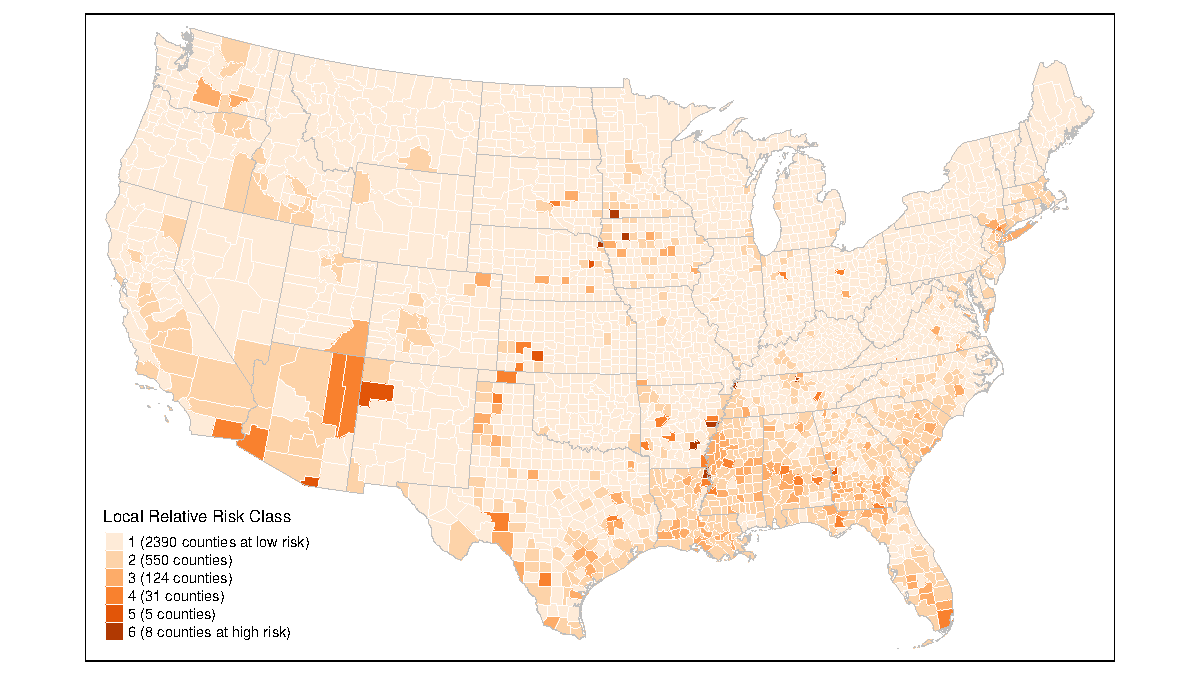
\includegraphics{C:/Users/gshanleybarr/Desktop/RPr-Chakraborty-2021/results/figures/map local relative risk score-1.pdf}

Next, map the cluster relative risk scores for comparison. Note that
following the original study classification methodology, counties
outside of clusters are assigned the lowest risk class of \texttt{1}.

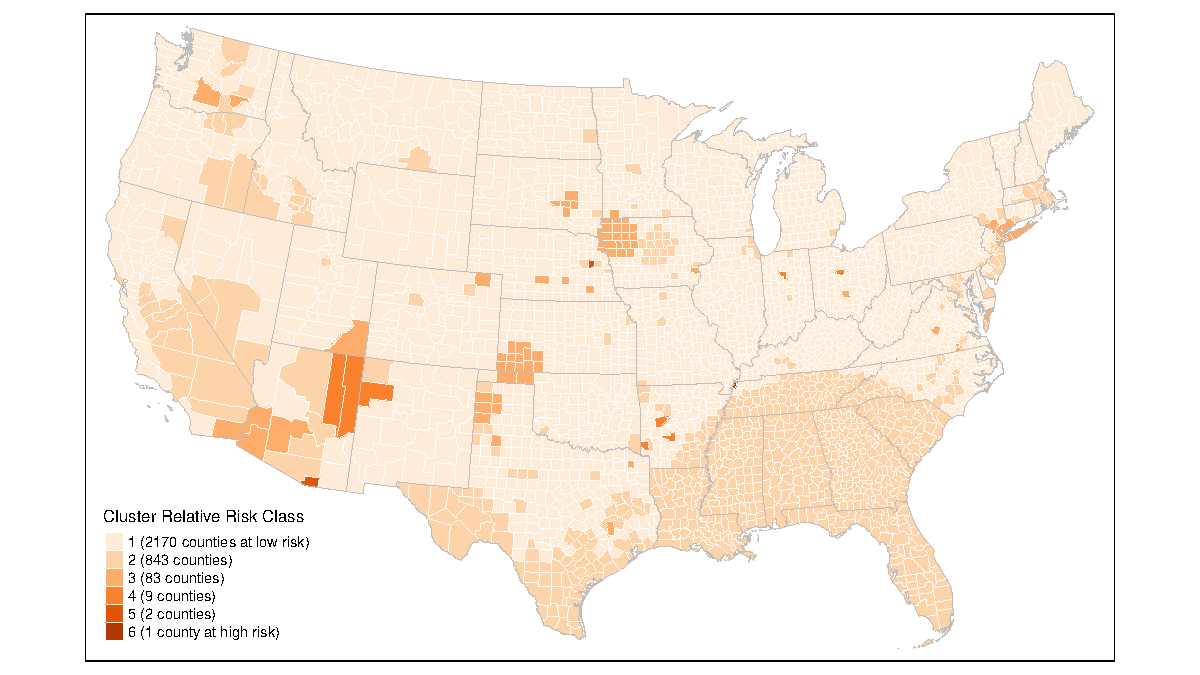
\includegraphics{C:/Users/gshanleybarr/Desktop/RPr-Chakraborty-2021/results/figures/map-cluster-relative-risk-classes-1.pdf}

Comparing the cluster and local relative risk classifications for
regions like the Southeast, it is apparent that some areas of high risk
are represented with large clusters that have an averaging effect on the
cluster-based relative risk score. This effect is more pronounced for
clusters with low compactness (e.g.~the Southeast cluster stretched over
the ``black belt'' region from Louisiana and Arkansas to Georgia) than
clusters with higher compactness (e.g.~New York City) because the
circular shape of clusters includes more low-risk counties.

\hypertarget{compare-clusters}{%
\subsubsection{Compare clusters}\label{compare-clusters}}

The original study did not directly report any results from the
Kulldorff spatial scan statistic. However, the Kulldorff cluster
relative risk scores were combined with states to create clusters for
GEE models, hereafter called ``GEE clusters''. The original study
reported \texttt{102} unique GEE clusters having a range of \texttt{1}
to \texttt{245} counties in each cluster.

In order to compare results, we first create cluster IDs as combinations
of the state ID and COVID relative risk class. The first clustering ID
(State) and second clustering score (COVID relative risk class) were
combined to form IDs for each unique combination of state and relative
risk class. Then, we find the number of unique clusters and frequency
counties per cluster in our reproduction study for comparison to the
original study.

\begin{verbatim}
## 111 unique clusters based on spatialEpi CLUSTER relative risk
\end{verbatim}

\begin{verbatim}
##    Min. 1st Qu.  Median    Mean 3rd Qu.    Max. 
##    1.00    2.00    7.00   27.56   50.50  159.00
\end{verbatim}

We failed to reproduce the same configuration of GEE clusters as the
original study, finding 9 more clusters than the original study and a
much smaller maximum cluster of 159 counties compared to 245 counties.

\hypertarget{reproduce-kulldorff-spatial-scan-statistic-in-satscan}{%
\subsubsection{Reproduce Kulldorff spatial scan statistic in
SaTScan}\label{reproduce-kulldorff-spatial-scan-statistic-in-satscan}}

\textbf{Unplanned deviation for reproduction}: Upon failing to reproduce
an identical number of GEE clusters using SpatialEpi in R, we reproduced
the procedure in the free but not open SaTScan software, using the
current software version 10.1. The input data files (\texttt{case},
\texttt{Coordinates.geo}, and \texttt{Population.pop}), and output data
files (\texttt{sat\_scan\_rpr.txt}, \texttt{sat\_scan\_rpr.col.shp}, and
\texttt{sat\_scan\_rpr.gis.shp}) are found in the
\texttt{data/derived/public/satscan} directory. The
\texttt{sat\_scan\_rpr.txt} file reports the model parameters used in
addition to results.

Although it is not ideal to intercede with this unplanned deviation at
this step, is the first step in the methodology following the Kulldorff
spatial scan statistic with a result reported in the original
publication.

First, load and verify whether our SaTScan reproduction data compares to
the author-provided SaTScan data.

\begin{verbatim}
## 96 reproduced relative risk observations
## 96 author-provided relative risk observations
\end{verbatim}

\begin{verbatim}
## 96 reproduced relative risk values match the original author's relative risk values
\end{verbatim}

Our SaTScan results exactly reproduced the author-provided SaTScan
results data.

\hypertarget{map-satscan-spatial-clusters}{%
\paragraph{Map SaTScan spatial
clusters}\label{map-satscan-spatial-clusters}}

Join the SaTScan results to \texttt{acs\_covid} for mapping and
analysis.

\begin{verbatim}
## Joining 96 records with 96 unique LOC_ID county values
\end{verbatim}

\textbf{Unplanned deviation for reproduction}: Visualize the spatial
distribution of the author-provided Kulldorff COVID-19 Clusters.

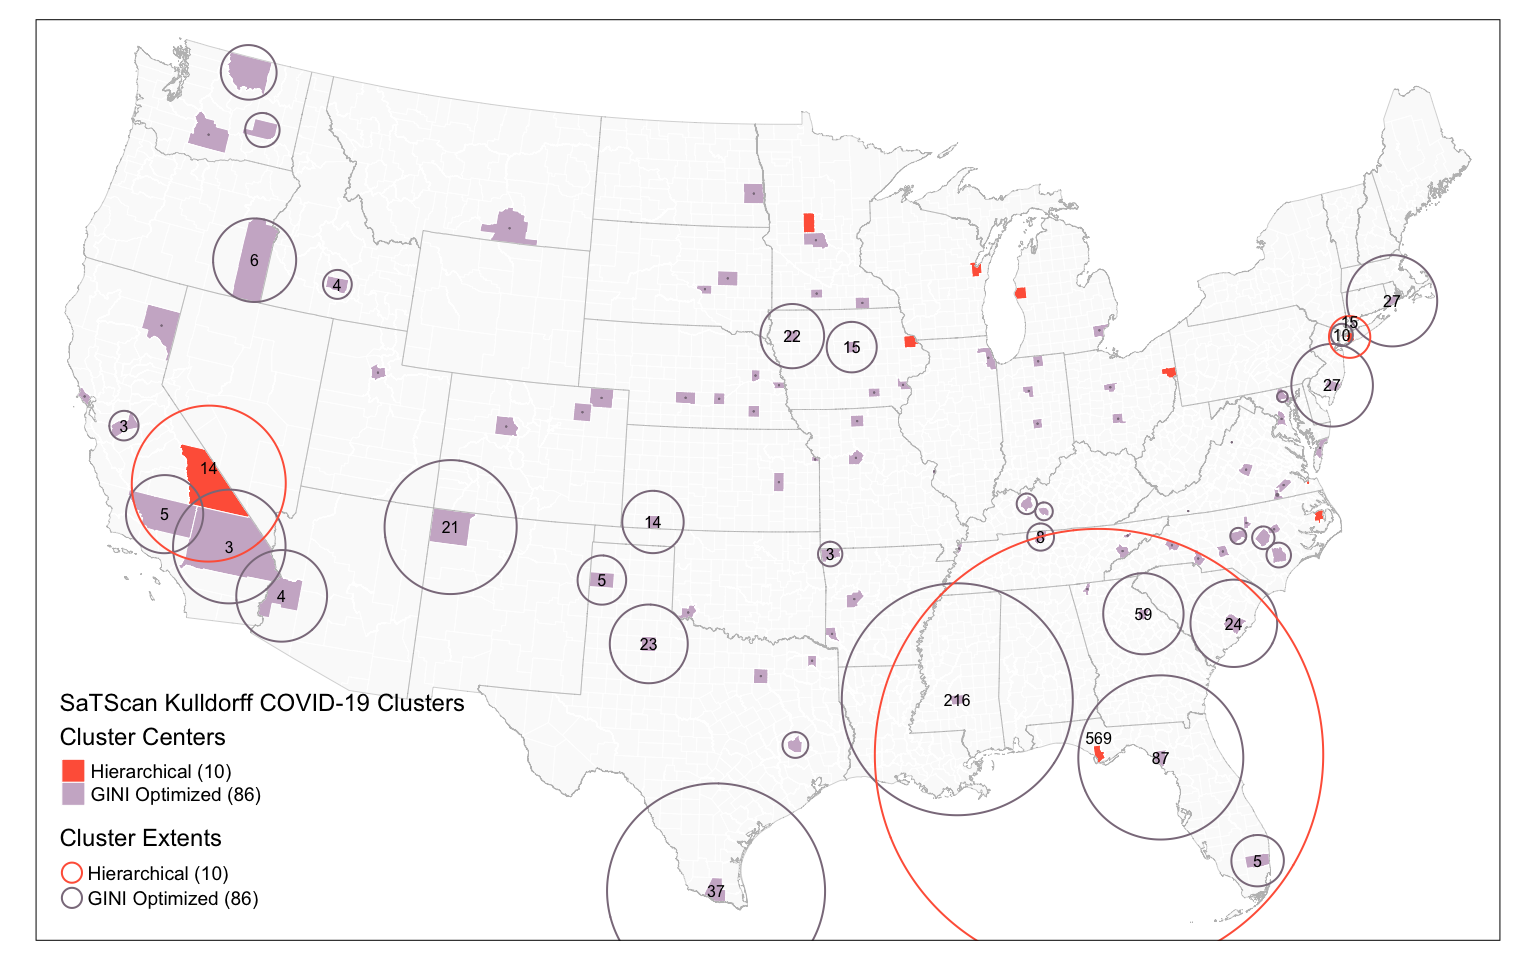
\includegraphics{C:/Users/gshanleybarr/Desktop/RPr-Chakraborty-2021/results/figures/map--author-clusters-1.pdf}

In the map above, clusters containing only one county have no visible
circle. Clusters containing two counties are encircled, but have no
label. Clusters containing three or more counties are encircled and
labelled with the number of counties.

Note that this version of data only includes the 96 counties defining
cluster centers, visualized with fill colors above. The data excludes
all of the non-center counties in clusters with more than one county.
The extent of these larger clusters is visualized by unfilled circles
defined by cluster radii.

Additionally, the SaTScan software confusingly merges two sets of
clusters in the results when the user uses the (default) option for
GINI-optimized clusters. One set of results is a hierarchical
non-overlapping set of clusters. These clusters are noted with
\texttt{GINI\_CLUST\ =\ F} in the results. The second set of results is
a set of hierarchical non-overlapping clusters designed to maximize the
GINI coefficient of inequality between counties within clusters and
counties outside of clusters. These clusters are noted with
\texttt{GINI\_CLUST\ =\ T} in the results.

Merged together as they are, the two sets of secondary clusters overlap
one another geographically, causing ambiguity in terms of which
cluster-based relative risk score should be used at each location.

\textbf{Unplanned deviation for reproduction}: Can we also use these
reproduced SaTScan results to exactly reproduce the author-reported
frequency of original GEE classes and maximum counties per class? If the
results match, it will confirm that the problems identified above have
propagated through the original study analysis.

\begin{verbatim}
## 102 unique clusters based on spatialEpi CLUSTER relative risk
\end{verbatim}

\begin{verbatim}
##    Min. 1st Qu.  Median    Mean 3rd Qu.    Max. 
##    1.00    1.00    3.00   29.99   58.75  245.00
\end{verbatim}

Using SaTScan Kulldorff clusters, we have exactly reproduced the
author-reported frequency of original GEE classes and maximum counties
per class. We have confirmed that the original study used the
\emph{cluster relative risk} of the \emph{center county} of each
cluster, including both the \emph{hierarchical} and
\emph{GINI-optimized} sets of clusters.

\hypertarget{compare-satscan-clusters-to-spatialepi-clusters}{%
\paragraph{Compare SaTScan clusters to SpatialEpi
clusters}\label{compare-satscan-clusters-to-spatialepi-clusters}}

\textbf{Unplanned Deviation for Reanalysis:} At this point it is clear
that the best decision will be to shift from a \emph{reproduction} study
to a \emph{reanalysis} study, intentionally altering methodological
decisions to achieve a more valid outcome. We prefer to include
\emph{all counties} contained in each cluster, and to use only \emph{one
set of non-overlapping clusters}, as produced by the \texttt{SpatialEpi}
algorithm.

Given the shifting goal, how sensitive is this study to the choice of
computational environment for the Kulldorff scan statistics? To answer
this question, we must load the local SaTSCan results inclusive of all
counties within clusters, filter the results to focus on the standard
hierarchical set of clusters, and compare the spatial distributions of
the SaTScan and SpatialEpi results.

\begin{verbatim}
## SaTScan combined GIS output has 1306 records with 922 unique county values
\end{verbatim}

\begin{verbatim}
## SaTScan Hierarchical clusters include 605 records with 605 unique county values
\end{verbatim}

\begin{verbatim}
## SaTScan GINI-optimized clusters include 701 records with 701 unique county values
\end{verbatim}

It was necessary to divide the Hierarchical clusters from the GINI
clusters to avoid duplicates and geographic overlap.

Compare the SaTScan Hierarchical clusters to the SpatialEpi clusters.

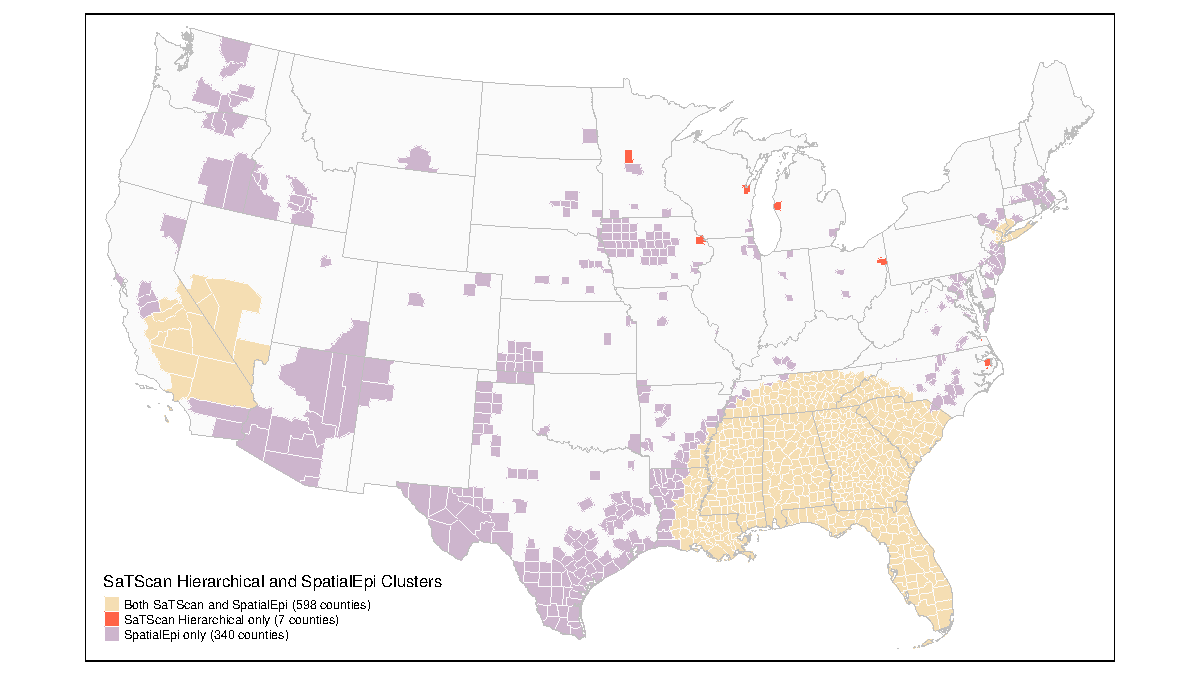
\includegraphics{C:/Users/gshanleybarr/Desktop/RPr-Chakraborty-2021/results/figures/hierarchical-cluster-comparison-map-1.pdf}

The two methods only agree on the definition of the largest clusters in
distant regions. Thereafter, SpatialEpi detects many secondary clusters
in the vicinity of the largest ones, while SaTScan detects seven
isolated and low-probability counties.

Compare the SaTScan GINI Optimized clusters to the SpatialEpi clusters.

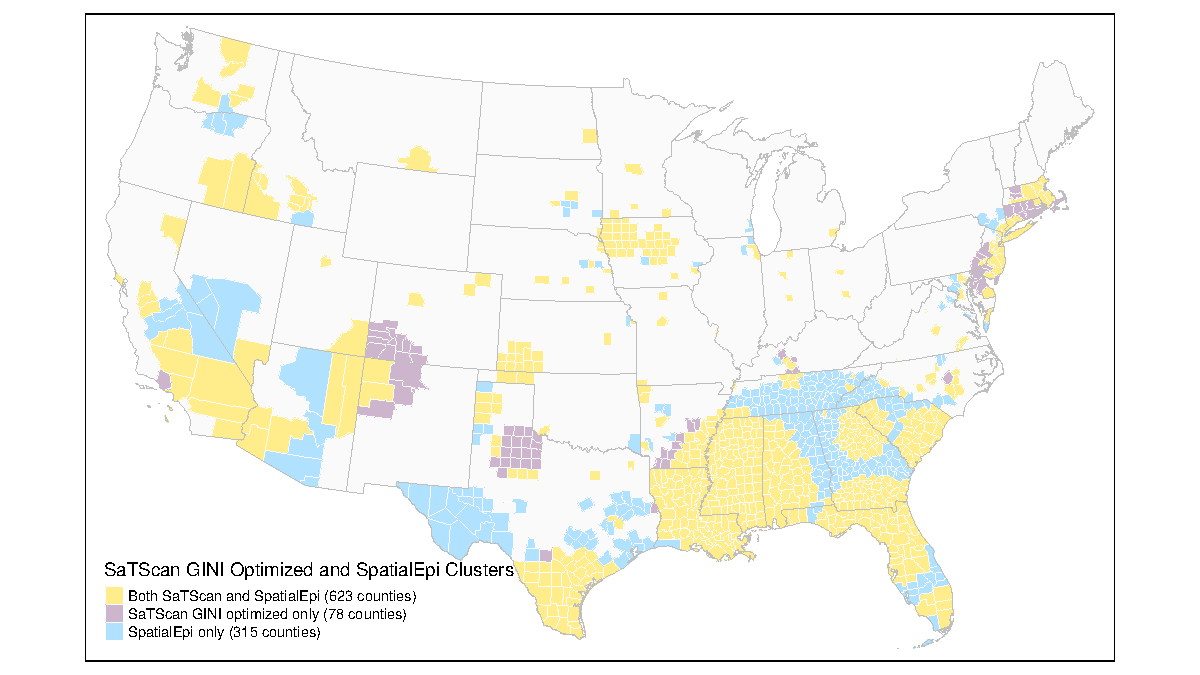
\includegraphics{C:/Users/gshanleybarr/Desktop/RPr-Chakraborty-2021/results/figures/gini-cluster-comparison-map-1.pdf}

There is more agreement overall between SpatialEpi and SaTScan GINI
Optimized clusters. The two algorithms agree the most for smaller and
less significant clusters above the 95\% confidence threshold. Because
the SaTScan clusters are more limited in size, SaTScan detects several
smaller clusters with gaps in place of the largest SpatialEpi clusters.

Keeping in mind that the final analysis uses a classification of cluster
relative risk for GEE models, are there important differences between
the two results with regard to classification of risk? We can check by
calculating cluster relative risk classes based on the SaTScan GINI
clusters, and cross-tabulating with the SpatialEpi risk classes.

\begin{table}

\caption{\label{tab:compare-spatialepi-satscan}COVID-19 Risk Class by County}
\centering
\begin{tabular}[t]{>{}l|>{\centering\arraybackslash}p{3em}|>{\centering\arraybackslash}p{3em}|>{\centering\arraybackslash}p{3em}|>{\centering\arraybackslash}p{3em}|>{\centering\arraybackslash}p{3em}|>{\centering\arraybackslash}p{3em}}
\hline
\multicolumn{1}{c|}{SpatialEpi} & \multicolumn{6}{c}{SatScan} \\
\cline{1-1} \cline{2-7}
  & 1 & 2 & 3 & 4 & 5 & 6\\
\hline
\textbf{1} & 2092 & 78 & 0 & 0 & 0 & 0\\
\hline
\textbf{\textbf{2}} & \textbf{306} & \textbf{528} & \textbf{9} & \textbf{0} & \textbf{0} & \textbf{0}\\
\hline
\textbf{3} & 7 & 6 & 69 & 1 & 0 & 0\\
\hline
\textbf{4} & 1 & 3 & 0 & 5 & 0 & 0\\
\hline
\textbf{5} & 1 & 0 & 0 & 0 & 1 & 0\\
\hline
\textbf{6} & 0 & 0 & 0 & 0 & 0 & 1\\
\hline
\end{tabular}
\end{table}

Indeed, SpatialEpi has identified more than 300 counties with above
normal risk that were not identified by SaTScan. Meanwhile, SaTScan
identified 78 counties with above normal risk that were not identified
by SpatialEpi.

The maps and crosstabulation above indicate that there are important
differences between the SaTScan and SpatialEpi computational
environments for calculating secondary clusters.

We summarize our understanding of the computational differences for
default settings below, based on close examination of our software
outputs, technical documentation for SaTScan, and the documentation and
code repository for SpatialEpi.

\begin{longtable}[]{@{}
  >{\centering\arraybackslash}p{(\columnwidth - 6\tabcolsep) * \real{0.2500}}
  >{\centering\arraybackslash}p{(\columnwidth - 6\tabcolsep) * \real{0.2500}}
  >{\centering\arraybackslash}p{(\columnwidth - 6\tabcolsep) * \real{0.2500}}
  >{\centering\arraybackslash}p{(\columnwidth - 6\tabcolsep) * \real{0.2500}}@{}}
\toprule\noalign{}
\begin{minipage}[b]{\linewidth}\centering
\end{minipage} & \begin{minipage}[b]{\linewidth}\centering
SaTScan Hierarchical
\end{minipage} & \begin{minipage}[b]{\linewidth}\centering
SaTScan GINI
\end{minipage} & \begin{minipage}[b]{\linewidth}\centering
SpatialEpi
\end{minipage} \\
\midrule\noalign{}
\endhead
\bottomrule\noalign{}
\endlastfoot
possible shapes & circle (default) or ellipse & circle (default) or
ellipse & circle \\
possible cluster centers & locations with rates \textgreater{} normal &
locations with rates \textgreater{} normal & all locations \\
maximum cluster size & 50\% of cases & varies, not exceeding 50\% of
cases & 50\% of population \\
maximum \emph{p} of cluster & 1.00 & 1.00 & 0.05 \\
distance & spherical great circle & spherical great circle & spherical
equidistant cylindrical projection \\
\end{longtable}

To further interrogate the differences in sets of secondary clusters, we
must understand that theoretically each location (county), may be the
center of many different circular clusters defined by different radii,
starting with a radius of 0 and the one county at the center, and
expanding until the maximum cluster size is reached.

\textbf{SaTScan Hierarchical Clusters}

\begin{itemize}
\tightlist
\item
  Select locations (counties) with above-normal COVID incidence rates
\item
  For each location, find log-likelihood of all possible cluster sizes
  (from minimum of 2 cases to maximum of 50\% of cases) with \emph{p}
  \textless{} 1
\item
  For each location, select the cluster with the maximum log-likelihood,
  resulting in one possible cluster for each location with above-normal
  COVID incidence rates
\item
  Sort the remaining clusters by log-likelihood from greatest to least
\item
  Select the most likely cluster
\item
  Select secondary clusters by iterating over the remaining clusters,
  adding new clusters to the set of secondary clusters if they do not
  geographically overlap any of the clusters already identified as most
  likely or secondary (pg 68).
\end{itemize}

\textbf{SaTScan GINI-Optimized Clusters}

\begin{itemize}
\tightlist
\item
  Follow the same procedure as SaTScan Hierarchical clusters, but
  iterate the procedure with different maximum cluster sizes. By default
  the cluster sizes include 1, 2, 3, 4, 5, 6, 8, 10, 12, 15, 20, 25, 30,
  35, 40, 45, and 50 percent of cases. With the default setting, the
  result is 17 different sets of clusters.
\item
  For each set of clusters, calculate the GINI coefficient of the
  COVID-19 incidence inside the clusters vs outside the clusters.
\item
  Select the set of clusters with the highest GINI coefficient (i.e.~the
  most difference between COVID-19 incidence inside the clusters vs
  outside the clusters).
\end{itemize}

\textbf{SpatialEpi Clusters}

\begin{itemize}
\tightlist
\item
  For all locations, calculate the log likelihood of all the possible
  clusters below the maximum cluster size (50\% of population)
\item
  Select the clusters with \emph{p} \textless{} 0.05
\item
  Sort the remaining clusters by log-likelihood from greatest to least
  (line 186)
\item
  Select the most likely cluster
\item
  Select secondary clusters by iterating over the remaining clusters,
  adding new clusters to the set of secondary clusters if they do not
  geographically overlap any of the clusters already identified as most
  likely or secondary (line 199).
\end{itemize}

The differences between these three approaches have very significant
impacts on the results (see the differences in results in the
\textbf{two maps} above) and it is impossible to control for all of the
differences with the available parameters. Most fundamentally, SaTScan
develops sets of secondary clusters from a universe of just one most
likely cluster per location with no default limitation its statistical
significance, whereas SpatialEpi may consider multiple possible cluster
sizes for each location with a default limitation of maximum 0.05
\emph{p} for each cluster. These fundamental differences are evident in
the spatial distribution of clusters. For example, New York City is the
most likely cluster in all analyses. For counties near New York, the
radius of the most likely cluster is large and geographically overlaps
New York City. Therefore, if only the most significant cluster radius is
considered as a possible secondary cluster for counties near New York
City, all such clusters are disqualified by their geographical overlap.
This is what happens in the SaTScan Hierarchical Clusters model, for
which the next nearest clusters are in Ohio and Virginia. In the SaTScan
GINI-optimized model, the maximum cluster size is apparently smaller,
such that the most likely cluster in New York City is also smaller. This
change allows for two other non-overlapping secondary clusters in Rhode
Island and New Jersey. In contrast, the SpatialEpi algorithm still
considers a variety of possible cluster sizes for each county, allowing
for detection of smaller clusters adjacent to more significant ones.

Of course, the \emph{relative risk} score of each cluster is contingent
on the cluster size, so each difference in geographic configuration of
clusters also impacts the cluster risk classification of individual
locations. The most stable results are for the most likely clusters in
distinct regions (New York City, Southeast U.S., Southern California \&
Nevada), while the most variability appears for secondary clusters close
enough for their most likely radius to overlap the more likely clusters.
The circular shape could be considered a major limitation of Kulldorff
cluster detection, for which the SaTScan methodology enhances the
limitation by constraining the possibility of nearby clusters while the
SpatialEpi methodology can detect smaller adjacent secondary clusters.

The high significance threshold in the default SaTScan analysis allows
the inclusion of many small clusters with low likelihoods, adding noise
to the results. This could be controlled by overriding the maximum
\emph{p} value parameter. Combining all of the default parameters,
SaTSCan includes small clusters of relatively low-risk counties in the
Midwest, but excludes relatively high-risk counties adjacent to the
major clusters of New York, the Southeast, and Southern
California/Nevada. This problem does not exist in the SpatialEpi
implementation, and the SpatialEpi parameter \emph{alpha level}
parameter cannot be practically increased to \texttt{1} to match the
SatSCan default. This is because SpatialEpi does not filter counties by
those with local relative risk greater than 1---therefore an \emph{alpha
value} of \texttt{1} results in \emph{all} counties being included as
clusters.

In sum, there are three construct validity issues with the original
study's COVID-19 high-risk clusters as implemented in SaTScan.

\begin{enumerate}
\def\labelenumi{\arabic{enumi}.}
\tightlist
\item
  Two sets of overlapping secondary clusters are included in the SaTScan
  output: hierarchical clusters and clusters optimized by GINI
  coefficient.
\item
  Only the 96 counties at the center of a cluster are considered in the
  risk classification.
\item
  The geographic patterns and cluster relative risk scores of secondary
  clusters are limited to circles or ellipses and are apparently
  sensitive to both the geographic shape and situation of high-risk
  clusters and to subjective decisions in parameters and algorithms.
\end{enumerate}

\hypertarget{preprocess-data-for-gee-modelling}{%
\subsection{Preprocess data for GEE
modelling}\label{preprocess-data-for-gee-modelling}}

\textbf{Unplanned deviation for reanalysis}: Based on the three
observations above, we think that it would be more valid to choose one
set of secondary clusters based on a single method rather than combining
a set of hierarchical clusters with a set of GINI optimized clusters. We
also think that it would be more valid to include risk levels for all
counties within a cluster (i.e.~all counties within any of the circles
above), rather than only the county at the center of a cluster. Finally,
we think it would be more valid to treat clusters as a single category
rather than five tiers of above-normal risk.

To complete the reproduction/reanalysis study, we will therefore
calculate and compare multiple versions of the GEE models:

\begin{enumerate}
\def\labelenumi{\arabic{enumi}.}
\tightlist
\item
  Original study results
\item
  Original study data in geepack
\item
  SpatialEpi cluster classification in geepack
\item
  SpatialEpi binary clusters in geepack
\end{enumerate}

\hypertarget{unique-gee-cluster-ids}{%
\subsubsection{Unique GEE cluster IDs}\label{unique-gee-cluster-ids}}

First, calculate GEE cluster IDs.

We have already calculated: - \texttt{rp\_clusID} based on our
SpatialEpi clusters - \texttt{ss\_clusID} based on our SaTScan cluster
centers, and shown to be identical to the original author's data -
\texttt{gini\_clusID} based on our SaTScan GINI-optimized clusters

\hypertarget{filter-and-standardize-data}{%
\subsubsection{Filter and standardize
data}\label{filter-and-standardize-data}}

Second, filter the data for non-zero COVID-19 rates and z-score
standardize the independent variables. This accomplishes step 10 of the
workflow diagram.

\textbf{Unplanned deviation for reproduction:} We assumed that we should
filter for COVID rates \textgreater{} 0 first and then calculate
z-scores, however after comparing data in the next code block, we
realized that the original study had \emph{first} calculated z-scores
and \emph{then} filtered for COVID rates \textgreater{} 0. Therefore, to
align with the original study, in the next code block we first calculate
z-scores and then filter for COVID rates \textgreater{} 0.

Compare independent variables for GEE models by subtracting the original
values from the reproduced values, and finding the average and standard
deviation of difference for each variable.

\begin{verbatim}
## Summary of difference between reproduction independent variables and original independent variables
\end{verbatim}

\begin{verbatim}
## Mean:
\end{verbatim}

\begin{verbatim}
##              z_white_pct              z_black_pct             z_native_pct 
##                        0                        0                        0 
##              z_asian_pct              z_other_pct     z_non_hisp_white_pct 
##                        0                        0                        0 
##               z_hisp_pct z_non_hisp_non_white_pct               z_bpov_pct 
##                        0                        0                        0 
##               z_apov_pct               z_pct_5_17              z_pct_18_34 
##                        0                        0                        0 
##              z_pct_35_64              z_pct_65_74                 z_pct_75 
##                        0                        0                        0 
##               z_male_pct             z_female_pct 
##                        0                        0
\end{verbatim}

\begin{verbatim}
## 
## Standard deviation:
\end{verbatim}

\begin{verbatim}
##              z_white_pct              z_black_pct             z_native_pct 
##                    0.000                    0.000                    0.000 
##              z_asian_pct              z_other_pct     z_non_hisp_white_pct 
##                    0.001                    0.001                    0.000 
##               z_hisp_pct z_non_hisp_non_white_pct               z_bpov_pct 
##                    0.000                    0.000                    0.000 
##               z_apov_pct               z_pct_5_17              z_pct_18_34 
##                    0.000                    0.001                    0.001 
##              z_pct_35_64              z_pct_65_74                 z_pct_75 
##                    0.000                    0.000                    0.000 
##               z_male_pct             z_female_pct 
##                    0.000                    0.000
\end{verbatim}

When we had filtered for COVID rates \textgreater{} 0 first and then
z-score standardized second, the means of differences ranged from -0.012
to 0.004, and standard deviations of differences ranged from 0.000 to
0.016.

After changing the order to first z-score standardize and then filter
for COVID rates \textgreater{} 0, we observed no mean difference between
our reproduced variables and the original variables, and we find no
standard deviation \textgreater{} 0.001 for the difference between
reproduction independent variables and original variables. There are no
major differences between the independent variables.

\hypertarget{save-final-derived-data}{%
\paragraph{Save final derived data}\label{save-final-derived-data}}

Optionally, you may save the preprocessed data to
\texttt{data/raw/public/gee\_data.gpkg}

Optionally, you may load the preprocessed data from
\texttt{data/raw/public/gee\_data.gpkg}

\hypertarget{gee-models}{%
\subsection{GEE models}\label{gee-models}}

The generalized estimating equation (GEE) models were used to test
association between intra-categorical rates of disability and COVID-19
incidence rates while accounting for spatial clustering. A separate
hypothesis was formulated for each type of subcategorization of PwDs,
numbered H2.1 through H2.5 in Table 4.

As specified by the author, ``GEEs extend the generalized linear model
to accommodate clustered data, in addition to relaxing several
assumptions of traditional regression (i.e., normality)''. Additionally,
the author noted that ``clusters of observations must be defined based
on the assumption that observations within a cluster are correlated
while observations from different clusters are independent.'' All five
GEE models were specified with exchangeable correlation matrices, gamma
distributions, and logarithmic link function. These specifications were
chosen after testing each alternative and choosing the models with the
best quasilikelihood under the independence model criterion (QIC).

This accomplishes the step 11 of the workflow diagram.

Generalized Estimating Equation parameters:

``The \textbf{`exchangeable' correlation matrix} was selected for the
results reported here, since this specification yielded the best
statistical fit based on the QIC (quasi- likelihood under the
independence) model criterion.'' (Chakraborty 2021, Methods paragraph 5)

``The \textbf{gamma distribution} with \textbf{logarithmic link
function} was chosen for all GEEs since this model specification
provided the lowest QIC value.'' (Chakraborty 2021, Methods paragraph 5)

\hypertarget{original-table-2}{%
\subsubsection{Original Table 2}\label{original-table-2}}

Load digitized version of Table 2 from the original publication.

\begin{table}

\caption{\label{tab:load-table2}Original Publication Table 2}
\centering
\begin{tabular}[t]{c|c|c|c|c|c|c}
\hline
term & estimate & std.error & conf.low & conf.high & wald\_chi\_square & p\_stars\\
\hline
Race model intercept & 7.106 & 0.083 & 6.997 & 7.322 & 7465.214 & 2\\
\hline
White & -0.203 & 0.020 & -0.242 & -0.164 & 102.958 & 2\\
\hline
Black & 0.111 & 0.016 & 0.079 & 0.143 & 46.214 & 2\\
\hline
Native American & 0.051 & 0.009 & 0.033 & 0.069 & 31.438 & 2\\
\hline
Asian & 0.080 & 0.018 & 0.046 & 0.115 & 21.060 & 2\\
\hline
Other race & 0.077 & 0.017 & 0.044 & 0.115 & 21.030 & 2\\
\hline
Ethnicity model intercept & 7.186 & 0.083 & 7.023 & 7.348 & 7525.648 & 2\\
\hline
Non-Hispanic White & -0.237 & 0.022 & -0.280 & -0.194 & 116.954 & 2\\
\hline
Hispanic & 0.119 & 0.031 & 0.058 & 0.180 & 14.708 & 2\\
\hline
Non-Hispanic non-White & 0.118 & 0.016 & 0.086 & 0.149 & 53.248 & 2\\
\hline
Poverty model intercept & 7.183 & 0.072 & 7.043 & 7.324 & 10066.930 & 2\\
\hline
Below poverty level & 0.148 & 0.022 & 0.105 & 0.190 & 46.913 & 2\\
\hline
Above poverty level & -0.267 & 0.023 & -0.312 & -0.222 & 134.297 & 2\\
\hline
Age model intercept & 7.242 & 0.076 & 7.093 & 7.391 & 9093.179 & 2\\
\hline
Age 5-17 & 0.047 & 0.016 & 0.016 & 0.078 & 8.732 & 2\\
\hline
Age 18-34 & 0.038 & 0.022 & -0.005 & 0.081 & 3.008 & 0\\
\hline
Age 35-64 & -0.026 & 0.023 & -0.071 & 0.019 & 1.300 & 0\\
\hline
Age 65-74 & -0.089 & 0.021 & -0.131 & -0.047 & 17.597 & 2\\
\hline
Age 75 or more & -0.108 & 0.020 & -0.148 & -0.069 & 29.479 & 2\\
\hline
Biological sex model intercept & 7.223 & 0.072 & 7.081 & 7.365 & 9963.672 & 2\\
\hline
Male & -0.298 & 0.028 & -0.353 & -0.243 & 113.460 & 2\\
\hline
Female & 0.153 & 0.029 & 0.097 & 0.209 & 28.577 & 2\\
\hline
\end{tabular}
\end{table}

\hypertarget{gee-function}{%
\subsubsection{GEE Function}\label{gee-function}}

Define a function for calculating and summarizing five GEE models

\hypertarget{original-clusters-and-original-covid-19-rate}{%
\subsubsection{Original Clusters and Original COVID-19
Rate}\label{original-clusters-and-original-covid-19-rate}}

Calculate GEE models with: - Clustering: SaTScan cluster centers \&
State ID - Dependent variable: original COVID-19 incidence (including
errors).

\begin{table}

\caption{\label{tab:gee-original-clusters-original-incidence}Original Cluster IDs and Original COVID-19 Incidence}
\centering
\begin{tabular}[t]{c|c|c|c|c|c|c}
\hline
term & estimate & std.error & conf.low & conf.high & stars & p.value\\
\hline
Race model intercept & 6.757 & 0.020 & 6.718 & 6.796 & 2 & 0.000\\
\hline
White & -0.201 & 0.026 & -0.251 & -0.150 & 2 & 0.000\\
\hline
Black & 0.281 & 0.020 & 0.242 & 0.321 & 2 & 0.000\\
\hline
Native American & 0.019 & 0.023 & -0.025 & 0.064 & 0 & 0.402\\
\hline
Asian & 0.064 & 0.024 & 0.016 & 0.112 & 2 & 0.008\\
\hline
Other race & 0.112 & 0.019 & 0.076 & 0.149 & 2 & 0.000\\
\hline
Ethnicity model intercept & 6.742 & 0.020 & 6.704 & 6.780 & 2 & 0.000\\
\hline
Non-Hispanic White & -0.226 & 0.026 & -0.277 & -0.175 & 2 & 0.000\\
\hline
Hispanic & 0.137 & 0.017 & 0.105 & 0.170 & 2 & 0.000\\
\hline
Non-Hispanic non-White & 0.278 & 0.019 & 0.241 & 0.315 & 2 & 0.000\\
\hline
Poverty model intercept & 6.816 & 0.021 & 6.774 & 6.858 & 2 & 0.000\\
\hline
Below poverty level & 0.240 & 0.027 & 0.186 & 0.293 & 2 & 0.000\\
\hline
Above poverty level & -0.303 & 0.030 & -0.362 & -0.245 & 2 & 0.000\\
\hline
Age model intercept & 6.820 & 0.021 & 6.779 & 6.862 & 2 & 0.000\\
\hline
Age 5-17 & 0.069 & 0.028 & 0.015 & 0.123 & 1 & 0.013\\
\hline
Age 18-34 & 0.029 & 0.034 & -0.038 & 0.097 & 0 & 0.395\\
\hline
Age 35-64 & 0.015 & 0.043 & -0.069 & 0.099 & 0 & 0.722\\
\hline
Age 65-74 & -0.044 & 0.042 & -0.126 & 0.039 & 0 & 0.298\\
\hline
Age 75 or more & -0.169 & 0.029 & -0.227 & -0.112 & 2 & 0.000\\
\hline
Biological sex model intercept & 6.814 & 0.021 & 6.772 & 6.855 & 2 & 0.000\\
\hline
Male & -0.402 & 0.042 & -0.484 & -0.319 & 2 & 0.000\\
\hline
Female & 0.298 & 0.044 & 0.212 & 0.385 & 2 & 0.000\\
\hline
\end{tabular}
\end{table}

\hypertarget{original-clusters-and-corrected-covid-19-rate}{%
\subsubsection{Original Clusters and Corrected COVID-19
Rate}\label{original-clusters-and-corrected-covid-19-rate}}

Calculate GEE models with: - Clustering: SaTScan cluster centers \&
State ID - Dependent variable: reproduced COVID-19 incidence (corrected
errors).

\begin{table}

\caption{\label{tab:gee-original-clusters-reproduced-incidence}Original Cluster IDs and Reproduced COVID-19 Incidence}
\centering
\begin{tabular}[t]{c|c|c|c|c|c|c}
\hline
term & estimate & std.error & conf.low & conf.high & stars & p.value\\
\hline
Race model intercept & 6.755 & 0.020 & 6.716 & 6.794 & 2 & 0.000\\
\hline
White & -0.213 & 0.024 & -0.261 & -0.165 & 2 & 0.000\\
\hline
Black & 0.284 & 0.020 & 0.244 & 0.325 & 2 & 0.000\\
\hline
Native American & 0.016 & 0.023 & -0.029 & 0.062 & 0 & 0.480\\
\hline
Asian & 0.055 & 0.028 & 0.001 & 0.110 & 1 & 0.048\\
\hline
Other race & 0.109 & 0.019 & 0.073 & 0.146 & 2 & 0.000\\
\hline
Ethnicity model intercept & 6.740 & 0.020 & 6.702 & 6.779 & 2 & 0.000\\
\hline
Non-Hispanic White & -0.238 & 0.024 & -0.285 & -0.191 & 2 & 0.000\\
\hline
Hispanic & 0.132 & 0.016 & 0.100 & 0.164 & 2 & 0.000\\
\hline
Non-Hispanic non-White & 0.281 & 0.019 & 0.243 & 0.318 & 2 & 0.000\\
\hline
Poverty model intercept & 6.816 & 0.021 & 6.774 & 6.858 & 2 & 0.000\\
\hline
Below poverty level & 0.241 & 0.028 & 0.186 & 0.295 & 2 & 0.000\\
\hline
Above poverty level & -0.311 & 0.030 & -0.370 & -0.252 & 2 & 0.000\\
\hline
Age model intercept & 6.820 & 0.021 & 6.779 & 6.862 & 2 & 0.000\\
\hline
Age 5-17 & 0.074 & 0.028 & 0.019 & 0.130 & 2 & 0.009\\
\hline
Age 18-34 & 0.026 & 0.035 & -0.042 & 0.095 & 0 & 0.449\\
\hline
Age 35-64 & 0.009 & 0.043 & -0.075 & 0.092 & 0 & 0.838\\
\hline
Age 65-74 & -0.041 & 0.042 & -0.124 & 0.041 & 0 & 0.327\\
\hline
Age 75 or more & -0.176 & 0.029 & -0.233 & -0.118 & 2 & 0.000\\
\hline
Biological sex model intercept & 6.815 & 0.021 & 6.774 & 6.856 & 2 & 0.000\\
\hline
Male & -0.401 & 0.042 & -0.484 & -0.319 & 2 & 0.000\\
\hline
Female & 0.292 & 0.044 & 0.206 & 0.377 & 2 & 0.000\\
\hline
\end{tabular}
\end{table}

\hypertarget{gini-clusters-and-fixed-covid-19-rate}{%
\subsubsection{GINI Clusters and Fixed COVID-19
Rate}\label{gini-clusters-and-fixed-covid-19-rate}}

Calculate GEE models with: - Clustering: Reproduced SaTScan GEE clusters
\& State ID - Dependent variable: reproduced COVID-19 incidence (fixed
errors).

\begin{table}

\caption{\label{tab:gee-gini-clusters-reproduced-incidence}Reproduced SaTScan GINI Cluster IDs and Reproduced COVID-19 Incidence}
\centering
\begin{tabular}[t]{c|c|c|c|c|c|c}
\hline
term & estimate & std.error & conf.low & conf.high & stars & p.value\\
\hline
Race model intercept & 6.769 & 0.020 & 6.730 & 6.809 & 2 & 0.000\\
\hline
White & -0.210 & 0.024 & -0.258 & -0.162 & 2 & 0.000\\
\hline
Black & 0.278 & 0.018 & 0.242 & 0.314 & 2 & 0.000\\
\hline
Native American & 0.028 & 0.021 & -0.013 & 0.070 & 0 & 0.180\\
\hline
Asian & 0.054 & 0.021 & 0.014 & 0.094 & 2 & 0.009\\
\hline
Other race & 0.098 & 0.017 & 0.065 & 0.130 & 2 & 0.000\\
\hline
Ethnicity model intercept & 6.753 & 0.020 & 6.714 & 6.793 & 2 & 0.000\\
\hline
Non-Hispanic White & -0.236 & 0.024 & -0.284 & -0.189 & 2 & 0.000\\
\hline
Hispanic & 0.127 & 0.016 & 0.096 & 0.158 & 2 & 0.000\\
\hline
Non-Hispanic non-White & 0.272 & 0.018 & 0.237 & 0.307 & 2 & 0.000\\
\hline
Poverty model intercept & 6.833 & 0.022 & 6.789 & 6.876 & 2 & 0.000\\
\hline
Below poverty level & 0.243 & 0.025 & 0.195 & 0.292 & 2 & 0.000\\
\hline
Above poverty level & -0.303 & 0.030 & -0.361 & -0.244 & 2 & 0.000\\
\hline
Age model intercept & 6.840 & 0.022 & 6.798 & 6.882 & 2 & 0.000\\
\hline
Age 5-17 & 0.071 & 0.025 & 0.022 & 0.120 & 2 & 0.005\\
\hline
Age 18-34 & 0.023 & 0.030 & -0.036 & 0.083 & 0 & 0.447\\
\hline
Age 35-64 & 0.026 & 0.036 & -0.044 & 0.096 & 0 & 0.467\\
\hline
Age 65-74 & -0.040 & 0.037 & -0.113 & 0.032 & 0 & 0.273\\
\hline
Age 75 or more & -0.179 & 0.029 & -0.235 & -0.122 & 2 & 0.000\\
\hline
Biological sex model intercept & 6.833 & 0.021 & 6.791 & 6.874 & 2 & 0.000\\
\hline
Male & -0.399 & 0.042 & -0.481 & -0.317 & 2 & 0.000\\
\hline
Female & 0.297 & 0.043 & 0.214 & 0.381 & 2 & 0.000\\
\hline
\end{tabular}
\end{table}

\hypertarget{spatialepi-clusters-and-fixed-covid-19-rate}{%
\subsubsection{SpatialEpi Clusters and Fixed COVID-19
Rate}\label{spatialepi-clusters-and-fixed-covid-19-rate}}

Calculate GEE models with: - Clustering: Reproduced SpatialEpi clusters
\& State ID - Dependent variable: reproduced COVID-19 incidence (fixed
errors).

\begin{table}

\caption{\label{tab:gee-spatialepi-clusters-reproduced-incidence}Reproduced SpatialEpi Cluster IDs and Reproduced COVID-19 Incidence}
\centering
\begin{tabular}[t]{c|c|c|c|c|c|c}
\hline
term & estimate & std.error & conf.low & conf.high & stars & p.value\\
\hline
Race model intercept & 6.755 & 0.020 & 6.716 & 6.795 & 2 & 0.000\\
\hline
White & -0.204 & 0.024 & -0.250 & -0.157 & 2 & 0.000\\
\hline
Black & 0.265 & 0.021 & 0.225 & 0.305 & 2 & 0.000\\
\hline
Native American & 0.021 & 0.023 & -0.024 & 0.065 & 0 & 0.367\\
\hline
Asian & 0.051 & 0.020 & 0.011 & 0.090 & 1 & 0.011\\
\hline
Other race & 0.086 & 0.018 & 0.050 & 0.122 & 2 & 0.000\\
\hline
Ethnicity model intercept & 6.743 & 0.020 & 6.704 & 6.781 & 2 & 0.000\\
\hline
Non-Hispanic White & -0.230 & 0.024 & -0.276 & -0.184 & 2 & 0.000\\
\hline
Hispanic & 0.115 & 0.016 & 0.083 & 0.146 & 2 & 0.000\\
\hline
Non-Hispanic non-White & 0.267 & 0.019 & 0.229 & 0.305 & 2 & 0.000\\
\hline
Poverty model intercept & 6.817 & 0.021 & 6.775 & 6.859 & 2 & 0.000\\
\hline
Below poverty level & 0.219 & 0.029 & 0.162 & 0.277 & 2 & 0.000\\
\hline
Above poverty level & -0.285 & 0.031 & -0.346 & -0.224 & 2 & 0.000\\
\hline
Age model intercept & 6.823 & 0.022 & 6.781 & 6.866 & 2 & 0.000\\
\hline
Age 5-17 & 0.063 & 0.023 & 0.018 & 0.108 & 2 & 0.006\\
\hline
Age 18-34 & 0.032 & 0.035 & -0.037 & 0.101 & 0 & 0.359\\
\hline
Age 35-64 & -0.004 & 0.041 & -0.085 & 0.076 & 0 & 0.914\\
\hline
Age 65-74 & -0.025 & 0.041 & -0.105 & 0.055 & 0 & 0.540\\
\hline
Age 75 or more & -0.160 & 0.027 & -0.214 & -0.107 & 2 & 0.000\\
\hline
Biological sex model intercept & 6.816 & 0.021 & 6.774 & 6.858 & 2 & 0.000\\
\hline
Male & -0.368 & 0.039 & -0.445 & -0.292 & 2 & 0.000\\
\hline
Female & 0.266 & 0.041 & 0.185 & 0.347 & 2 & 0.000\\
\hline
\end{tabular}
\end{table}

\hypertarget{compare-gee-results}{%
\subsubsection{Compare GEE results}\label{compare-gee-results}}

\textbf{Unplanned deviation for reanalysis}: Generate dot-and-whisker
plot of coefficients for each of the model variations for efficient
visual comparison of coefficients across each model.

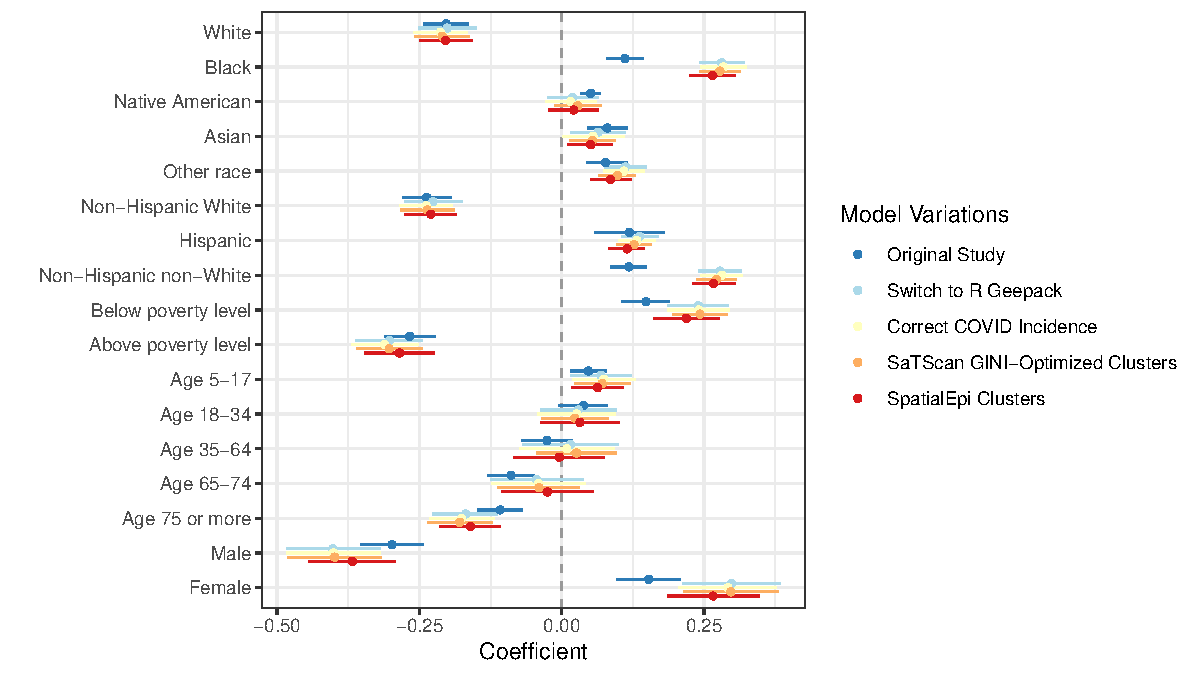
\includegraphics{C:/Users/gshanleybarr/Desktop/RPr-Chakraborty-2021/results/figures/dotwhisker-comparison-1.pdf}

The figure above illustrates five model variations, starting with the
results published in the original study. The next two models make
incremental adjustments to the research design and are most compatible
with the goals of a reproduction study.

The greatest differences were produced using the same input data in
different computational environments, caused by switching the
computational environment from SPSS to geepack in R. This switch
decreased the magnitude of most coefficients, reducing the positive
Hispanic coefficient below its original confidence interval and
increasing the negative Above poverty level and Male coefficients to the
limits of their original confidence intervals.

Compared to the change in computational environment, fixing the error in
the COVID-19 incidence rate of 13 counties had very little effect on
coefficient estimates.

Our more significant adjustments could be considered reanalyses, in
which we re-conceptualized COVID-19 clusters first as all counties
included in SaTScan GINI-Optimized clusters, and second as all counties
included in SpatialEpi clusters. These two changes further decreased the
magnitude of most coefficients as they likely more effectively fulfilled
the purpose of controlling for spatial dependence. The shifts were most
signficant for the Ethnicity model, in which the Hispanic and
Non-Hispanic white coefficients lost magnitude beyond the original
confidence interval and the Hispanic coefficient is no longer
significant. Secondarily, the negative Above poverty level and Male
coefficients both increased beyond the range of the original confidence
intervals.

Overall, we can see that some coefficients remained significant and
robust to changes in computational environment, data errors, and
clustering criteria. Robustly positive coefficients included Black,
Native American, Non-Hispanic non-White, Below poverty level, and
Female. The Asian and Age 5-17 coefficients also remained just above 0.
All of these categories of people with disabilities would be considered
intersectional with factors of vulnerability. Conversely, some robustly
negative coefficients indicate people with disabilities intersecting
with non-vulnerable identities, such as white, Non-Hispanic White, Above
poverty level, and Male. Counter-intuitively, the two coefficients for
elderly people with disability were also robustly negative.

\hypertarget{interpret-gee-model}{%
\subsubsection{Interpret GEE Model}\label{interpret-gee-model}}

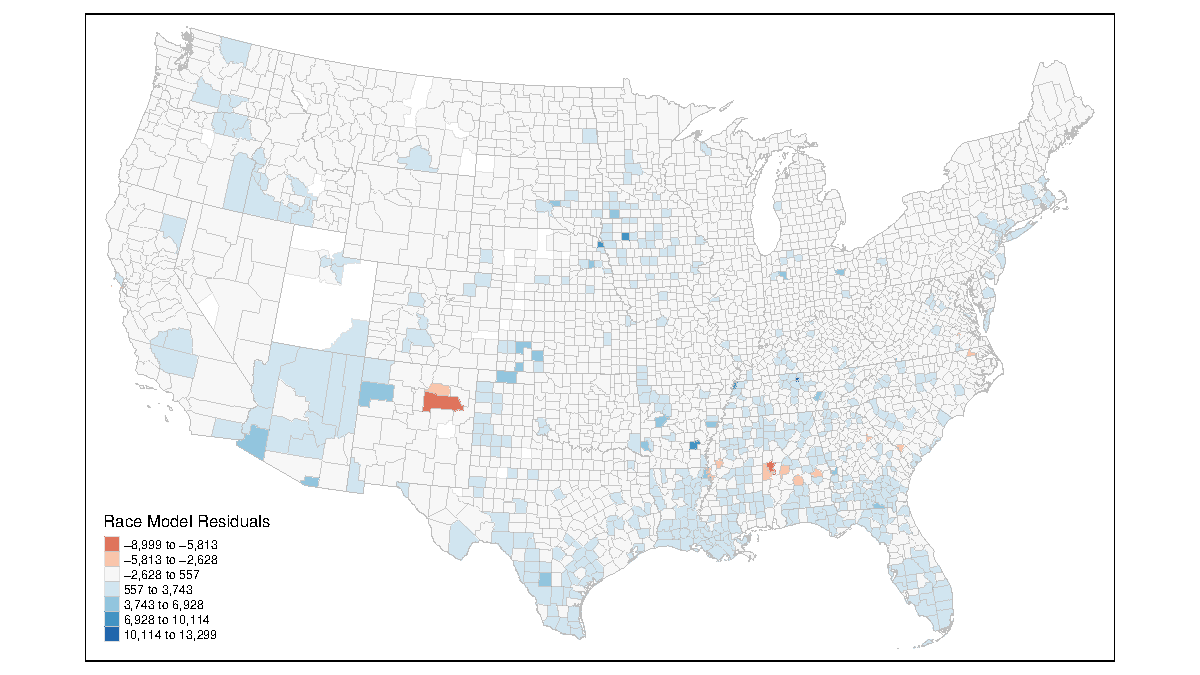
\includegraphics{C:/Users/gshanleybarr/Desktop/RPr-Chakraborty-2021/results/figures/map-residuals-1.pdf}

Calculate variance, covariance, correlation, and weights

Map each county's weight in GEE model.

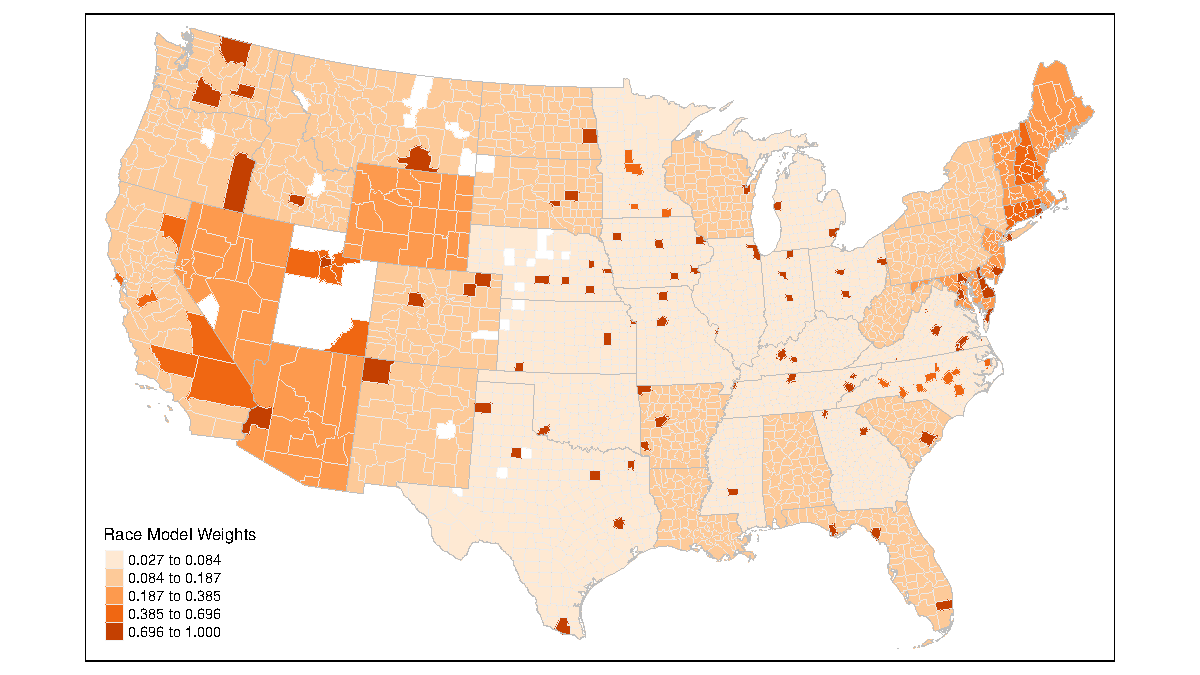
\includegraphics{C:/Users/gshanleybarr/Desktop/RPr-Chakraborty-2021/results/figures/map-weights-1.pdf}

\hypertarget{discussion}{%
\section{Discussion}\label{discussion}}

\hypertarget{bias-and-threats-to-validity}{%
\subsection{Bias and threats to
validity}\label{bias-and-threats-to-validity}}

Given the research design and primary data to be collected and/or
secondary data to be used, discuss common threats to validity and the
approach to mitigating those threats, with an emphasis on geographic
threats to validity.

\textbf{Edge effects} were not accounted for in the analysis.

The analysis created \textbf{spatial subgroups} based on \textbf{spatial
clustering}. The purpose of this grouping was to control for
\textbf{spatial heterogeneity} between regions (defined as states) and
\textbf{spatial correlation} within regions using GEE models. The
spatial subgroups based on state and COVID-19 risk were specified in the
attribute transformation subsection above.

This analysis accounted for \textbf{first order spatial effects} of
regional difference by including states in the clustering criteria for
GEE models. The analysis accounted for some \textbf{second order spatial
effects} by including a relative risk score for COVID-19 spatial
clusters in the clustering criteria for GEE models. The analysis did not
account for \textbf{spatial anisotropies}, as the Kulldorff spatial scan
statistic was constrained to circular non-directional clusters.

The study used a cross-sectional design, aggregating cases across the
full \textbf{temporal extent} from 1/22/2020-8/1/2020. The
\textbf{temporal support} was inconsequential, as both the COVID-19
cases and disability sociodemographic data were aggregated across time
for the full temporal extent. \textbf{Temporal effects} were not
conceptualized, measured, or accounted for. There is potential for error
and uncertainty in areas experiencing rapid socio-demographic change due
to the \textbf{temporal coverage} of the socio-demographic data, as it
was derived from ACS estimates from 2014 to 2018, prior to the onset of
the COVID-19 pandemic.

There was no documentation of any \textbf{data exclusion} based on
attribute criteria in the original study. No \textbf{outliers} were
analyzed or accounted for in the study. No \textbf{weights} were applied
in the study.

\hypertarget{unplanned-deviations}{%
\subsection{Unplanned deviations}\label{unplanned-deviations}}

Some minor unplanned deviations stemmed from small operational errors or
the constraints of a short journal article for describing the data and
methodology of a research project. These deviations could be resolved
with computational notebooks, and include the resolution of some missing
data for Rio Arriba County, New Mexico, mapping disability rates, and
resolving data errors

We planned to test the independent variables for normality prior to
using the Pearson's r correlation coefficient for bivariate tests of
correlation between the independent variables and COVID-19 incidence
rates. Most of the independent variables had significantly non-normal
distributions; and therefore our reproduction has used the nonparametric
Spearman's rank correlation coefficient for bivariate tests of
correlation between the independent variables and COVID-19 incidence
rates. In order to better understand the geographic patterns underlying
the correlations between disability and COVID-19, we also visualized
disability rates by county.

The original study did not directly report details for the results of
the Kulldorff spatial scan statistic for COVID-19 clusters beyond the
number of clusters detected. In order to compare our reproduction using
the SpatialEpi package to the original study using SaTScan software, we
also ran the spatial scan statistic in SaTScan. SaTScan produced three
outputs: 1. text file report of the analysis with information on each
cluster 1. vector layer of circle polygons with the center and radius of
each cluster, ID of the county at the center of the cluster, and a
relative risk score for the cluster. The layer contained one circular
polygon feature for each cluster (see figure 4), identifying only the
county at the center of the cluster. 1. vector layer of points of the
centroids of each county in any cluster, including a unique cluster ID,
relative risk score of the cluster, and relative risk score of the
location (the county).

We compared our results to the original publication, data files provided
by the author, and the number of clusters for GEE models. We exactly
reproduced the original author's data files using our data inputs and
SaTScan software. In order to better understand how the original
research used the Kulldorff spatial scan statistic, we decided to create
an additional map to visualize the spatial distributions of COVID-19
clusters resulting from SaTScan software. We created maps visualizing
the spatial clusters of COVID-19 incidence based on the output of
SpatialEpi and SaTScan. We discovered that the original study most
likely operationalized COVID-19 risk as the local relative risk of the
county at the center of the cluster using the vector layer of circle
polygons enumerated as the second output above. This operationalization
excluded all but the center county of each cluster and assigned the
other counties to the lowest risk category. For example, SaTScan
identified a circular cluster encompassing all of Rhode Island and most
of Massachusetts, Connecticut, and Long Island. However, the original
operationalization of COVID-19 risk only considered the relative risk of
the county at the center of the cluster: Washington County, Rhode
Island. All other counties were classified as minimal risk. We also
discovered that unlike SaTScan, the SpatialEpi package in R did not
calculate local or cluster relative risk.

Therefore, we changed our conceptualization of COVID-19 clusters to
include all counties within any cluster. We calculated relative risk for
localities (counties) and clusters as
\texttt{(incidence\ rate\ within\ the\ county)\ /\ (incidence\ rate\ outside\ of\ the\ county)}.
We calculated the Kulldorff spatial scan statistic in
\texttt{SpatialEpi} and then calculated local relative risk for any
county within any of the resulting clusters. Once we joined the spatial
clustering data to all counties with socio-demographic and COVID-19
data, we observed that all counties outside of any cluster had
\texttt{null} or \texttt{na} data for COVID-19 risk. We inspected the
original author's data to determine how to classify these counties, and
accordingly assigned them to the lowest risk class: \texttt{1}. We
created a map showing the relative risk score of each county (Figure 5)
for comparison with the original analysis and to assess its
appropriateness for GEE clusters. We proceeded to combine the local
COVID risk score with State ID's for use as the GEE clustering ID and to
run the GEE models.

At this point we observed the spatial heterogeneity of local relative
risk (Figure 5) and considered the original purpose of calculating
clusters and relative risk classes, which was to control for spatial
dependence within states and COVID-19 hotspots. Out of concern to
balance a need to control for spatial dependence while not accounting
for too much variation within the dependent variable, we decided to
re-conceptualize the classification of COVID risk using cluster-based
relative risk. To calculate the cluster relative risk, we created a list
of unique cluster IDs and extracted the counties contained within each
cluster from \texttt{SpatialEpi} output and calculated cluster relative
risk as:
\texttt{(incidence\ rate\ within\ the\ cluster)\ /\ (incidence\ rate\ outside\ of\ the\ cluster)}.
We then classified the cluster relative risk with the original method,
illustrated in Table 2. We re-classified the GEE clustering IDs based on
state and cluster relative risk class and recalculated the generalized
estimating equations using this alternative conceptualization of
COVID-19 risk.

Upon discovering different results in all of our reproduction GEE models
compared to the original study, we added new models to assess the extent
to which the different computational environment was causing differences
in our results. We therefore ran another set of the five GEE models
using data provided by the original author, expecting to find identical
results.

\hypertarget{rationale-for-updated-report}{%
\subsubsection{Rationale for updated
report}\label{rationale-for-updated-report}}

This is the second version of our reproduction report. The first,
registered at \url{https://doi.org/10.17605/OSF.IO/647EX} on July 22,
2022, represented our best knowledge of the study at that time.
Subsequently, we improved our approaches to reproduction studies by
revising pre-analysis plans and post-analysis reports into legible code
RMarkdown documents. This change prompted us to re-order some content to
flow more linearly with the sequencing required by code, and prompted us
to digitize (if necessary) and import results from the original research
into Rmarkdown for quantitative comparison to the reproduction study.
These comparisons led to further insights and research into
discrepancies between the original and reproduced Pearsons's
correlations between various forms of the Kulldorff spatial scan
statistic. We also discovered an improved method for comparing the
results of generalized linear models by plotting all of the model
results on a dot-wisker graph using the dotwhisker package.

\hypertarget{emilys-discussion}{%
\section{Emily's Discussion}\label{emilys-discussion}}

Our reproduction of the original study was partially successful, leading
to similar, but inexact results compared to the original study. A
portion of the inexactitude may be attributed to differences in the
computational environments. However, we have also reanalyzed the study
and tested its robustness by changing some research parameters. Our
results suggest support for the conclusions of the original study, but
also emphasize the importance of reproduction studies to critically
review the full details of the research design, to evaluate internal
validity, and to test for uncertainty and robustness to key parameters.

The choropleth map we made in the \textbf{first part} of the
reproduction analysis (Figure 2) reveals an identical spatial pattern to
that of the original study's Figure 1, confirming the equivalence of our
dependent variable with that of the original study. Both maps revealed
that COVID-19 cases were distributed unevenly across space. In
particular, cases were more prevalent in the southern part of the
country, in the metropolitan areas of the northeast, Chicago, and
California, and in some rural areas, including eastern Washington, New
Mexico, and Iowa. Prior to Chakraborty's bivariate analysis of
disability and COVID-19 incidence, we also mapped the spatial
distribution of disability (Figure 3). This spatial visual analysis
reveals many regions in which disability rates are high but COVID-19
incidence was still low, including rural New England, Appalachia, and
northern Michigan. Conversely, many hotspots of COVID-19 incidence had
low rates of disability, including metropolitan New England, South
Florida, and Chicago. The two spatial distributions help explain the
negative bivariate relationship between disability rates and COVID-19
incidence.

The summary statistics for the \textbf{second part} of the reproduction
analysis matched perfectly with those of the original study, confirming
that the reproduction uses identical original data. The original study
used Pearson's correlation to test bivariate relationship between
variables that are non-normally distributed, and we revised this to use
the nonparametric Spearman's correlation coefficient. Our reanalysis of
the correlations generally found identical directions and increased
magnitudes, confirming the bivariate correlations and significance
levels of most of the socio-demographic subcategories. However,
biological sex may not be correlated with COVID-19 incidence rates, as
the percentage of females with disabilities changes direction and
significance.

The Kulldorff spatial scan statistic varied significantly between the
original study and our reproduction and re-analysis with regards to
selection of secondary clusters, interpretation of clusters, and
relative risk scores. SatScan and SpatialEpi identify the same most
likely cluster, but different sets of secondary clusters. They also
employ slightly different distance calculations, where SatScan
calculates a great circle spherical distance and SpatialEpi approximates
a kilometer grid based on simplified conversions of latitude and
longitude degrees into a planar grid using kilometer units. SaTScan uses
GINI statistics to select secondary clusters which maximize the
difference between the population within clusters and the population
outside of clusters, allowing for geographic overlap and finding 96
total clusters. The original study used this default secondary cluster
selection method. SpatialEpi selects the most likely secondary clusters
while excluding clusters with any geographic overlap, finding 135 total
clusters. This difference of parameters and computational environment
explains the two different sets of clusters. The different sets of
secondary clusters largely agree in terms of the most likely cluster in
a region and diverge in terms of overlapping, small, and less likely
clusters.

The original study classified COVID risk using a local relative risk
score for the county at the center of each cluster (Figure 4).
Considering the relatively small number of clusters (102) compared to
counties (3108), this method implies that the majority of counties in
each state are classified as one low-risk cluster for the GEE analysis,
and the remaining 53 clusters were composed of just a few counties at
the centers of various COVID hotspots. When we extended the
interpretation of clusters to use the local relative risk score of any
county within a cluster (Figure 5), we find significantly more variance
in COVID risk within states, resulting in 139 unique GEE clusters.
However, this conceptualization apparently created GEE clusters defined
in part by an ordinal classification of the dependent variable -- COVID
incidence. Considering that the original motivation for using GEE models
was to account for spatial dependence within states (accounting for
COVID response policy) and within COVID hotspots (accounting for the
uneven geographic diffusion of the pandemic). Therefore, a cluster-based
relative risk classification seemed more appropriate than a local
county-based relative risk classification, by applying the same risk
level to the entire COVID cluster and allowing the GEE models to analyze
variance within the clusters. However, many of the most likely clusters
extend across multiple states (see Figure 6, especially the southern
states from Louisiana to South Carolina). This resulted in creation of
GEE clusters composed of every county within a state, amounting to 111
unique GEE clusters overall.

Our analysis of COVID-19 clusters in the context of controlling for
spatial dependence has revealed several challenges and limitations to
application of Kulldorff spatial scan statistics across different
computational environments. These include inconsistent methods for
determining secondary clusters, limitation to circular or ellipsoidal
cluster shapes, inclusion of single-county clusters, and choosing a
method to control for spatial dependence in COVID 19 risk without
controlling for too much of the variance in the dependent variable.
Ideally, we would have liked to use a GINI-based secondary cluster
detection to classify counties by their maximum cluster-based relative
risk score, but this particular conceptualization is not possible in
available R packages.

In the \textbf{third part} of our reproduction analysis, the results
from each the five GEE models were largely consistent with
Chakraborty's, suggesting robustness to modeling decisions with regards
to GEE clusters. However, a few independent variables exhibited
instability across models, suggesting weak or spurious relationships. We
ultimately modeled three different scenarios: 1. We reproduced the
original analysis with the original data while changing only the
computational environment to geepack in R. 2. We reproduced the
Kulldorff spatial scan in R and reanalyzed the data by applying a local
relative risk score to every county within any cluster. 3. We reproduced
the Kulldorff spatial scan in R and reanalyzed the data by applying a
cluster relative risk score to every county in a cluster.

We found that reproducing the analysis with \textbf{geepack} resulted in
slightly different GEE results than the original study, even when using
data provided by the author from the original study. This suggests that
the computational environments differ in their implementation of GEE, a
method for which there are multiple approaches to parameter estimation.
Still, the coefficients trend in the same direction with similar
magnitudes, with the exception of the 35-64 age group. In our model that
assigns local relative risk scores for all counties in clusters, the
coefficients are weaker while more of the variance in COVID-19 incidence
is accounted for in the GEE clustering method. When we moved to
cluster-level relative risk scores, the coefficients again performed
more similarly to the original publication. Although the results of the
original publication and the cluster-level relative risk model version
are similar, the model conceptualization is very different. The original
model excludes most counties from COVID-19 hotspots, assigning them the
lowest level of risk and inadvertently avoiding the problem of
controlling for too much variance in COVID-19 through definition of
clusters. Conversely, the reanalyzed cluster-based model includes most
counties in COVID-19 hotspots at the same risk level. The results are
similar because in both scenarios the majority of counties in each state
are aggregated into the same cluster.

Comparing across each version of the model, we observed that most
variables exhibit stability in the direction and magnitude of the
coefficients. However, some variables are less stable -- especially the
black and other race categories, Hispanic ethnicity, and some age groups
less affected by severe COVID-19 cases (18-34 and 35-64). Therefore,
these variables are more sensitive to the design of GEE clusters,
warranting further investigation to evaluate the internal validity of
these relationships with regard to the model assumptions of GEE.

We confirmed support for Chakraborty's conclusion that although the
overall disability percentage is negatively associated with confirmed
COVID-19 cases, intra-categorical analysis with geographic GEE
clustering reveals that socio-demographically disadvantaged PwDs were
significantly over-represented in counties with higher COVID-19
incidence. We found the same direction for each independent variable of
intra-categorical disability and COVID-19 incidence. However, we found
weaker significance levels for the Black category and the Hispanic or
Latino category. We found stronger significance levels for the 18-34 and
35-64 age categories. Differences in our results can be attributable to
our different approach to classifying relative risk scores and our
different computational environments.

Closer inspection of the clusters for the GEE models revealed a highly
skewed distribution of cluster sizes, with most clusters containing very
few counties and a few clusters containing 50 or more counties. GEE
weights observations based on the number of observations within a
cluster and the degree of correlation in the standard errors within
clusters. Therefore, counties within small clusters (e.g.~the counties
of Rhode Island or the few counties with high COVID risk classification)
will have much larger weights than counties within large clusters
(e.g.~counties with low risk classifications in large states). The
combination of very different cluster sizes and use of a clustering
criteria related to the dependent variable warrant further analysis with
alternative approaches to controlling for spatial dependence. We quickly
diagnosed whether the clustering method was significantly skewing the
estimated coefficients by running non-clustered generalized linear (GLM)
models for each of the hypotheses H2.1 through H2.5. Fortunately, we
found the GLM coefficients to be consistent, and in most cases stronger,
than the GEE model coefficients. Future replications of this research
should consider selecting an alternative inferential statistical model
which explicitly accounts for spatial dependence.

With regards to the \textbf{overall conclusions} and \textbf{research
design}, we agree with the original author's cautious interpretation
emphasizing ``county-level associations'' and the need for ``additional
data and analysis''. There are at least five sources of uncertainty in
this study: ecological fallacy, scale dependency, modifiable areal unit
problem, variable measurement, and spatial dependency. There is a risk
of ecological fallacy with this research design, whereby county-level
statistics for the whole population should not be interpreted as
definitive inferential proof of individual-level relationships,
especially for populations comprising no more than one third of any
county. Counties are not weighted by population. Therefore, in this
analysis a few people with disabilities in a rural county are
collectively weighted as one observation with equal weight to many
people with disabilities in an urban county as another observation.
There is a real possibility that the study findings are scale-dependent,
but it is also impossible to replicate the study using a finer spatial
support without also limiting the extent to one or more adjacent states
with sub-county data on COVID-19. The modifiable areal unit problem
(MAUP) may also be a source of uncertainty, especially when considering
the variable population sizes of counties, which all carry equal weights
in the analysis. Finally, there are well-known problems with the testing
and reporting of COVID-19 cases across time and space during the
pandemic in the United States, and there is also uncertainty in American
Community Survey (ACS) data, particularly when cross-tabulating multiple
demographic characteristics. This study partially mitigates measurement
uncertainty by aggregating data across time (more than one year of the
pandemic and the five-year ACS estimate) and into relatively large
geographic units (counties). The study accounts for spatial dependency
using the GEE models to cluster county observations by state and COVID
risk classification. However, the GEE method simply uses correlation
matrices to weight each county observation according to the number of
observations in its cluster and the overall within-cluster correlation
of standard errors. The spatial dependence between counties in different
clusters is not modelled, even if the counties are adjacent to each
other.

In sum, although some of our results differed from Chakraborty's because
of differences in analytical methods, conceptualizations, and
computational environments, our reproduction results still suggest that
PwDs are likely to experience multiple jeopardy based on the convergence
of their disability, racial/ethnic minority, and poverty status. We
reiterate Chakraborty's carefully limited interpretation emphasizing
county-level relationships and the need for additional data and
research, because the estimated relationship at the county level may not
hold at the individual level. Interpretation of the results were based
on aggregate statistics at the county level and on statistical methods
which produce approximate estimates, not inferences. Further work is
needed to reliably infer relationships between minority PwDs and
COVID-19 morbidity and mortality, especially at finer geographic scales.

\end{document}
